%%&latex
\documentclass[12pt]{article}
\usepackage{graphicx,psfrag,epsf}
\usepackage{graphicx}
\usepackage{natbib}

%\pdfminorversion=4
% NOTE: To produce blinded version, replace "0" with "1" below.
\newcommand{\blind}{0}

\setlength{\textheight}{24 cm}

% DON'T change margins - should be 1 inch all around.
\addtolength{\oddsidemargin}{-.5in}%
\addtolength{\evensidemargin}{-.5in}%
\addtolength{\textwidth}{1in}%
\addtolength{\textheight}{-.3in}%
\addtolength{\topmargin}{-.8in}%



\newcommand*{\lpath}{./}%
%\usepackage[cmex10]{amsmath, mathtools}
%\usepackage{amsmath,amssymb,amsbsy,amsfonts,amsthm}
\usepackage{amsmath,amssymb,amsbsy,amsfonts}
\usepackage{mathtools}
\usepackage{booktabs}
\usepackage{multirow}
\usepackage{bm}
\usepackage{enumerate}
\usepackage{url}
%\usepackage[ruled,vlined]{algorithm2e}
\usepackage{fancyvrb}
\usepackage{yfonts}
\usepackage{wrapfig}
\usepackage{subfigure}
\usepackage{tikz}
\usetikzlibrary{bayesnet}
\newcommand{\tikzmark}[1]{\tikz[overlay,remember picture] \node (#1) {};}
\usepackage{calc}%    For the \widthof macro
\usepackage{xparse}%  For \NewDocumentCommand


%% Variable de compilation
\newif\ifbeamer
\beamerfalse
\newcommand{\beamer}[2]{\ifbeamer #1 \else #2 \fi}
%%%

%\usepackage[latin1]{inputenc}
\usepackage[utf8]{inputenc} % manage utf8 encodage 
%\usepackage[english]{babel} % for french document ! dirty enumerate style,+ bad change rectangle colors for section linking.
\usepackage{fancyhdr} % for heading
\usepackage{listings}
\usepackage[colorlinks=true, urlcolor=blue]{hyperref} % url, link
\usepackage{graphicx}
\usepackage{geometry}

%\usepackage[cmex10]{amsmath, mathtools}
\usepackage{amsmath,amssymb,amsbsy,amsfonts,amsthm}
\usepackage{multirow}
\usepackage{bm}
\usepackage{enumerate}
\usepackage{url}
\usepackage[ruled,vlined]{algorithm2e}
\usepackage{fancyvrb}
\usepackage{yfonts}

\usepackage{wrapfig}
\usepackage{tikz}
    %\input{../tikz.conf}
    
\usetikzlibrary{bayesnet}
    
%%%%%%%%%%% Box 
\usepackage{calc}%    For the \widthof macro
\usepackage{xparse}%  For \NewDocumentCommand
\newcommand{\tikzmark}[1]{\tikz[overlay,remember picture] \node (#1) {};}

%%%%%%%%%% Math
\renewcommand{\text}{\textnormal}
\newcommand{\pr}{\mathbf{p}}
\newcommand{\E}{\mathbb{E}}
\newcommand{\divkk}{\mathbb{K}}
\newcommand{\entropy}{\mathbb{H}}
\newcommand{\gem}{\mathrm{GEM}}
\newcommand{\Mult}{\mathrm{Mult}}
\newcommand{\DP}{\mathrm{DP}}
\newcommand{\IBP}{\mathrm{IBP}}
\newcommand{\M}{\mathcal{M}}
\newcommand{\V}{\mathcal{V}}
\newcommand{\N}{\mathcal{N}}
    
\makeatletter
\NewDocumentCommand{\DrawBox}{s O{}}{%
    \tikz[overlay,remember picture]{
    	\IfBooleanTF{#1}{%
    		\coordinate (RightPoint) at ($(left |- right)+(\linewidth-\labelsep-\labelwidth,0.0)$);
    	}{%
    	\coordinate (RightPoint) at (right.east);
    }%
    \draw[red,#2]
    ($(left)+(-0.2em,0.9em)$) rectangle
    ($(RightPoint)+(0.2em,-0.3em)$);}
}

\NewDocumentCommand{\DrawBoxWide}{s O{}}{%
	\tikz[overlay,remember picture]{
		\IfBooleanTF{#1}{%
			\coordinate (RightPoint) at ($(left |- right)+(\linewidth-\labelsep-\labelwidth,0.0)$);
		}{%
		\coordinate (RightPoint) at (right.east);
	}%
	\draw[red,#2]
	($(left)+(-\labelwidth,0.9em)$) rectangle
	($(RightPoint)+(0.2em,-0.3em)$);}
}
\makeatother
%%%%% ! Box

\geometry{
      a4paper,
	    body={160mm,260mm},
	    left=25mm,top=20mm,
	    headheight=4mm,headsep=8mm,
        footskip=10mm,
        }
                                              

%%%%%%%%%%%%%%%%%%%%%%%%%%%%%%%%%%%%%%%%%%%%%%%%%%%%%%%%%%%%%%%%%%%%%%%%%%%%%%%%%%%%%%%%%%%%%%%%%%%%%%
%%%%% => Internal
%%%%%%%%%%%%%%%%%%%%%%%%%%%%%%%%%%%%%%%%%%%%%%%%%%%%%%%%%%%%%%%%%%%%%%%%%%%%%%%%%%%%%%%%%%%%%%%%%%%%%%

% itemize item def
%% \begin{itemize}\itemsep2pt % example space betwew item
%\renewcommand{\FrenchLabelItem}{\textbullet}
\renewcommand{\labelitemi}{$\bullet$}
\renewcommand{\labelitemii}{$\cdot$}
\renewcommand{\labelitemiii}{$\diamond$}
\renewcommand{\labelitemiv}{$\ast$}

% equation reference
\renewcommand{\theequation}{\thesection.\arabic{equation}}

%%%%%%%%%%%%%%%%%%%%%%%%%%%%%%%%%%%%%%%%%%%%%%%%%%%%%%%%%%%%%%%%%%%%%%%%%%%%%%%%%%%%%%%%%%%%%%%%%%%%%%
%%%%% => Alias
%%%%%%%%%%%%%%%%%%%%%%%%%%%%%%%%%%%%%%%%%%%%%%%%%%%%%%%%%%%%%%%%%%%%%%%%%%%%%%%%%%%%%%%%%%%%%%%%%%%%%%

% write code
\lstnewenvironment{C}[1]
{\lstset{language=C,
      frame=tBRl,
      basicstyle=\scriptsize,stringstyle=\emph,showstringspaces=false,
      numbers=left,numberstyle=\tiny,
      breaklines=true, columns=flexible, title={#1}}
}{}
      
%%%%%%%%%%%%%%%%%%%%%%%%%%%%%%%%%%%%%%%%%%%%%%%%%%%%%%%%%%%%%%%%%%%%%%%%%%%%%%%%%%%%%%%%%%%%%%%%%%%%%%
%%%%% => Preambles Pages
%%%%%%%%%%%%%%%%%%%%%%%%%%%%%%%%%%%%%%%%%%%%%%%%%%%%%%%%%%%%%%%%%%%%%%%%%%%%%%%%%%%%%%%%%%%%%%%%%%%%%%

\pagestyle{fancy}
\fancyhf{} % remove default headers
\fancyfoot[C]{\thepage}
\renewcommand{\footrulewidth}{0.3pt}
\renewcommand{\headrulewidth}{0.3pt}

%%%%%%%%%% Math
\renewcommand{\text}{\textnormal}
\newcommand{\ifm}{\texttt{ILFM}}
\newcommand{\imb}{\texttt{IMMSB}}
\newcommand{\pr}{P}
\newcommand{\p}{P}
\newcommand{\E}{\mathbb{E}}
\newcommand{\divkk}{\mathbb{K}}
\newcommand{\entropy}{\mathbb{H}}
\newcommand{\gem}{\mathrm{GEM}}
\newcommand{\Mult}{\mathrm{Mult}}
\newcommand{\DP}{\mathrm{DP}}
\newcommand{\IBP}{\mathrm{IBP}}
\newcommand{\M}{\mathcal{M}}
\newcommand{\V}{\mathcal{V}}
\newcommand{\N}{\mathcal{N}}
\newcommand{\mat}[1]{\mathbf{#1}}
\newcommand{\unit}{1\!\!1}

\newtheorem{definition}{Definition}[section]
\newtheorem{lemma}{Lemma}[section]
\newtheorem{proposition}{Proposition}[section]
\newtheorem{theorem}{Theorem}[section]
\newtheorem{corollary}{Corollary}[section]
\newtheorem{proof}{Proof}[section]



\begin{document}

\def\spacingset#1{\renewcommand{\baselinestretch}%
{#1}\small\normalsize} \spacingset{1}


%%%%%%%%%%%%%%%%%%%%%%%%%%%%%%%%%%%%%%%%%%%%%%%%%%%%%%%%%%%%%%%%%%%%%%%%%%%%%%

\if1\blind
{
  \title{\bf A study of stochastic mixed membership models for link prediction in social networks}
  \author{Author 1\thanks{
    The authors gratefully acknowledge \textit{please remember to list all relevant funding sources in the unblinded version}}\hspace{.2cm}\\
    Department of YYY, University of XXX\\
    and \\
    Author 2 \\
    Department of ZZZ, University of WWW}
  \maketitle
} \fi

\if0\blind
{
  \bigskip
  \bigskip
  \bigskip
  \begin{center}
    {\LARGE\bf A study of stochastic mixed membership models for link prediction in social networks}
\end{center}
  \medskip
} \fi

\bigskip
\begin{abstract}
We assess here whether standard stochastic mixed membership models are adapted for link prediction in social networks by studying how they handle homophily and preferential attachment. To do so, we first introduce formal definitions of these phenomena; we then study how stochastic mixed membership models relate to these definitions. Our theoretical analysis reveals that standard stochastic mixed membership models comply with homophily with the similarity that underlies them. For preferential attachment, the situation is more contrasted: if these models do not comply with global preferential attachment, their compliance to local preferential attachment depends on whether the memberships to latent factors are hard or soft, and in the latter case on whether the underlying latent factor distribution is bursty or not. We illustrate these elements on synthetic and real networks by using the generative properties of Bayesian model.
\end{abstract}

\noindent%
{\it Keywords:}  Hierarchical Bayesian Models, Random Graph, Machine Learning.
\vfill

\newpage
\spacingset{1.45} % DON'T change the spacing!

\section{Introduction}
\label{sec:introduction}
In recent years, several powerful relational learning models have been proposed to solve the problem commonly referred to as \textit{link prediction} that consists in predicting the likelihood of a future association between two nodes in a network \cite{Liben-Nowell07, HassanZaki11}. Among such models, the class of probabilistic, generative models has received much attention as such models can be used to both generate artificial networks and infer new links from existing ones. Two main class of models have been proposed and studied in the literature: the latent feature model \cite{BMF} and its non-parametric extension \cite{ILFRM}, and the mixed-membership stochastic block model \cite{MMSB} and its non parametric extensions \cite{iMMSB,diMMSB}. In this paper, we focus on this two model, and study some of its properties related to link prediction in social networks. 

Indeed, although drawn from a wide range of domains, most real world social networks exhibit common properties, such as the \textit{homophily}, \textit{preferential attachement} and \textit{small world} effects \cite{Newman2010, Barabasi2003}. 


A natural question that arises is thus whether or not models as IMMSB and ILFM comply with such properties. Link prediction model, typically learned or given, describe a set of nodes and links between them; Such data defines a random structure $Y$. Given that, we learn a model parameters $\hat \theta$, such that one can then predict the probability that a new link will be drawn between two given nodes of the network by studying the following quantity:
\begin{equation}
\p(y | \hat \theta)
\end{equation}
This quantity is called a predictive likelihood.


A question we ask in this setting is: \textit{Do link prediction models learned can generate networks with the homophily and preferential attachment}.

A second possible use of Bayesian models is as a pure generative model to generate artificial networks. In this setting, we study models properties based on their expectation over their random parameters, defined as follows:

\begin{equation}
\p(y) = \int_{\theta} \p(y,\theta) d\theta
\end{equation}
This quantity is know as the evidence for the data.

The question we ask ourselves in this setting is thus: \textit{Do link prediction models comply with the homophily and preferential attachment effects}.


The remainder of the paper is organized as follows. In the second section \ref{sec:background} we set up the probabilistic context of our analysis, Then in section \ref{sec:models} we present two general class of models in this settings know as class based models and feature based models. Then in section \ref{sec:homophily} and \ref{sec:burstiness} we propose respectively formal definition for the homophily and preferential effects and study how models comply with this propoerties. \textcolor{red}{Then section on feature dynamics and sparsity}. In section \ref{sec:experiments} we report an empirical study of the predictive performance on synthetic and real networks with regards to the properties. We conclude in the last section \ref{sec:concl}. 

\section{Models}
%\emph{Yet another view} ~\\
\label{sec:models}

As mentioned before, we focus in this study on two major representatives of the latent models used for link prediction in social networks, namely the latent feature model \cite{BMF} and the mixed-membership stochastic block model \cite{MMSB}. To be as general as possible, we consider non-parametric extensions of these models, respectively based on the Indian Buffet Process (IBP) and the Hierarchical Dirichlet Process (HDP). Similar extensions have already been considered in the past, {\it e.g.} through the Infinite Latent Feature model \cite{ILFRM} and through conditional random fields \cite{iMMSB} or a dynamic version of the Hierarchical Dirichlet Process \cite{diMMSB}.
%\textcolor{red}{To be completed - maybe second extension not considered yet}

We now briefly describe the two models retained.
%Our two chosen baseline use prior distributions that fall into the two major classes of discrete nonparametric priors. The Hierarchical Dirichlet Process (HDP) that generalizes the Latent Dirichlet Allocation (LDA) for infinite mixtures models. On the other hand, the Indian Buffet Process (IBP), which is the generalization of the Beta-Bernoulli compound distribution (ie Beta Process), which generates infinite binary matrices. The nonparametric models in their truncated version are equivalent to well-known models such as LDA, widely used for text analysis, and Mixed Membership Stochastic Blockmodel which is an adaptation of the latter for relational learning.~\\

%We adopt the following notation; if a matrix has a negative index superscripted, it indicates that the values corresponding to this index are excluded. A dot $\bm{.}$ in the index means that we marginalize over all possible values.

\subsection{Infinite Latent Feature Model (ILFM)}

In the latent feature model, each node is represented by a vector of binary features. The probability of linking two nodes is then based on a weighted similarity between their feature vectors, the weight matrix being generated according to a normal distribution. In its non-parametric version, the feature vectors are now generated according to an IBP, leading feature vectors of infinite dimensions (even though only a finite number of dimensions are actually active). The following steps summarizes this process:
%
\begin{enumerate}
\item Generate a feature matrix $\mat{F}_{N \times \infty}$ representing the feature vector of each node: $\mat{F} \sim \IBP(\alpha)$
\item Generate a weight matrix for each latent feature:\\
 $\mat{\phi}_{mn} \sim N(0, \sigma_w), \, m,n \in \mathbb{N}^{+*}$
\item Generate or not a link between any node $i$ and any node $j$ according to: 
%
\begin{equation}
y_{ij} \sim \mathrm{Bern}(\sigma(\mat{f}_{i} \mat{\Phi} \mat{f}_{j}^\top))
\label{eq:link-ilfm}
\end{equation}
\end{enumerate}
%
where $\sigma()$ is the sigmoid function, mapping $[-\infty, +\infty]$ values to [0,1], and where $y_{ij}$ is a binary variable indicating that a link has been generated ($y_{ij}=1$) or not ($y_{ij}=0$). We will denote by $\mat{Y}$ the $N \times N$ matrix with elements $y_{ij}$. Finally, $\mat{f}_{i}$ denotes the row vector corresponding to the $i^{th}$ row of $\mat{F}$.

This model makes use of two real hyper-parameters, one for the IBP process ($\alpha$), and one for the variance of the normal distribution underlying the weight matrix ($\sigma_w$). In the case of undirected networks, the matrices $\mat{Y}$ and $\mat{\Phi}$ are symmetric and only their upper (or lower) diagonal parts are generated. Lastly, both $\mat{F}$ and $\mat{\Phi}$ are infinite matrices. In practice however, one always deal with a finite number of latent features. A graphical representation of this model is given in Figure~\ref{fig:ilfrm}.

\begin{figure}[t]
	\centering
	\minipage{0.25\textwidth}\vspace{1cm}
	\scalebox{0.88}{
	\begin{tikzpicture}
  % Define nodes
  \node[obs]                      (y) {$y_{ij}$};
  \node[latent, left=1.2cm of y] (fi) {$\mat{f}_i$};
  \node[latent, right=1.2cm of y] (fj) {$\mat{f}_j$};
  \node[latent, above= of y]    (ibp) {$\mat{F}$};;
  \node[latent, below= of y, yshift=-0.3cm]   (W) {$\mat{\Phi}$};
  \node[const, left=0.7cm of ibp]   (a) {$\alpha$};
  \node[const, right=0.7cm of W]   (sw) {$\sigma_w$};

  % Connect the nodes
  \edge {fi,fj,W} {y} ;
  \edge[dashed] {ibp} {fi,fj} ;
  \edge {sw} {W} ; 
  \edge {a} {ibp} ; 

  % Plates
  \plate {yx} {(fj)(y)} {$N$} ;
  \plate[label={[label distance=-0.6cm]195:$N$}] {} {(fi)(y)(yx.north west)(yx.south west)} {} ;
  %\plate {} {(W)} {$K\times K$};
  %\plate {} {(fi)(y)(yx.north west)(yx.south west)} {$N$} ;
\end{tikzpicture}
}
	\endminipage
	\minipage{0.25\textwidth}
	\scalebox{0.88}{
		/home/dulac/Documents/workInProgress/networkofgraphs/papers/personal/figures/draw/mmsb2.tex}
	\endminipage
	\caption{The two graphical representations of (left) the latent feature model and (right) the latent class model. The difference between the two models lies in the way representations are associated to nodes: a fixed representation is used in the case of the latent feature model, whereas the representation in the latent class model varies according to the link considered.}
	\label{fig:ilfrm}
\end{figure}

Standard Gibbs sampling and Metropolis-Hastings algorithms can be used for inference in this model. We do not detail them here and refer the interested reader to \cite{ILFRM}.

%We here only provide the main updates, useful for the developments presented in the next sections, and refer the reader to \cite{IBP} for a detailed treatment. The Gibbs update for the matrix $\mat{F}$ are given by:
%%
%\begin{align}
%& P(f_{ik} = 1 \mid \mat{F}^{-ik}) = \frac{m_k^{-i}}{N} \nonumber \\
%& P(f_{ik} = 0 \mid \mat{F}^{-ik}) = 1 - \frac{m_k^{-i}}{N} \nonumber
%\end{align}
%%
%where $m_k^{-i}$ represents the number of active features $k$ for all nodes excluding node $i$, hence $m_k^{-i} = \sum_{j=1, j\neq i}^N f_{jk}$. $\mat{F}^{-ik}$ represents the matrix $\mat{F}$ without its element on the $i^{th}$ row and $k^{th}$ column.
%
%The learning of the weight matrix $W$ is computed using a Metropolis-Hasting algorithm in which each weight is sequentially sampled according to (\cite{IBP}): 
%%
%\begin{equation}
%P(\phi_{mn} \mid \mat{Y}, \mat{F}, \mat{\Phi}^{-mn}, \sigma_w) \propto P(\mat{Y} \mid \mat{F}, \mat{\Phi}) P(\phi_{mn} \mid \sigma_w) \nonumber
%\end{equation}
%%
%One can then choose a jumping distribution in the normal family (as for the prior), with a mean based on the previous sample:
%%
%\begin{equation} \label{eq:j_w}
%J(\phi_{mn}^* \mid \phi_{mn}) = \mathcal{N}(\phi_{mn}, \eta) \nonumber
%\end{equation}
%%
%where $\eta$ is a parameter controlling the acceptance ratio, $r_{\phi_{mn}\rightarrow \phi_{mn}^*}$, defined by:
%%
%\begin{equation} \label{eq:r_w}
%r_{\phi_{mn}\rightarrow \phi_{mn}^*} = \frac{ P(\mat{Y} \mid \mat{F}, \mat{\Phi}^*)P(\phi_{mn}^* \mid \sigma_w)J(\phi_{mn} \mid \phi_{mn}^*) }{ P(\mat{Y} \mid \mat{F}, \mat{\Phi})P(\phi_{mn} \mid \sigma_w)J(\phi_{mn}^* \mid \phi_{mn} )} \nonumber
%\end{equation}

\subsection{Infinite Mixed-Membership Stochastic Block Model (IMMSB)}

The MMSB model generates class membership distributions per node on the basis of a Dirichlet distribution. Then, for each connection between two nodes, a particular class for each node is first sampled from the class membership distribution, and the probability of connecting the two nodes is, as in the previous model, based on a Bernoulli distribution integrating the weight of the two classes. 

The non-parametric version parallels this development but considers, in lieu of the Dirichlet distribution, a hierarchical Dirichlet process, leading to the following generative model:
%
\begin{enumerate}
\item Generate the class membership matrix $\mat{F}_{N \times \infty}$:
   \begin{align}
    &\bm{\beta} \sim \gem(\gamma) \nonumber \\
    \mat{f}_i &\sim \DP(\alpha_0, \beta) \quad\text{ for }  i \in \{1, .., N\} \nonumber
   \end{align}
where $\gem$ denotes the Griffiths, ??? distribution over the set of natural numbers and $\DP$ a Dirichlet Process  \cite{HDP}.
\item Generate a weight matrix for each latent class:\\
\[ \phi_{mn} \sim \mathrm{Beta}(\lambda_0,\lambda_1), \, m,n \in \mathbb{N}^{+*} \]
\item For any node $i$ and any node $j$, choose a class from their class membership distribution and generate or not a link according to:
   \begin{align}
    z_{i \rightarrow j} &\sim \mbox{Cat}(\mat{f}_i) \nonumber \\
    z_{i \leftarrow j} &\sim \mbox{Cat}(\mat{f}_j) \nonumber \\
    y_{ij} &\sim \mathrm{Bern}(\phi_{z_{i \rightarrow j}f_{i \leftarrow j}})
    \label{eq:link-immsb}
   \end{align}
\end{enumerate}
%
We have this time four real hyper-parameters, two for the hierarchical Dirichlet process ($\gamma$ and $\alpha_0$) and two for the Beta distribution underlying the weight matrix ($\lambda_0$ and $\lambda_1$). As for the previous model, in the case of undirected networks, the matrices $\mat{Y}$ and $\mat{\Phi}$ are symmetric and only their upper (or lower) diagonal parts are generated; as before again, both $\mat{F}$ and $\mat{\Phi}$ are infinite matrices. A graphical representation of this model is given in Figure~\ref{fig:ilfrm}.

The inference is this model can be performed via collapsed Gibbs sampling updates. Most updates can be found in \cite{HDP} and \cite{diMMSB}. For completeness, we provide them in Appendix~\ref{sec:append}.
%%
%\begin{enumerate}
%\item If the class $k$ has already been observed:
%   \begin{align}
%    \pr(z_{ij} =k \mid \mat{F}^{-ij}) &\propto N_{ik}^{-ij} + \alpha_0 \beta_k
%%    \pr(f_{ji} =k \mid \mat{F}^{-ij}) &\propto N_{jk}^{-ij} + \alpha_0 \beta_k
%    \label{eq:update-immsb}
%   \end{align}
%\item In case of a new class $k_n$:
%   \begin{align}
%    \pr(z_{ij} =k_n \mid \mat{F}^{-ij}) &\propto \alpha_0 \beta_{k_n} \nonumber
%%    \pr(f_{ji} =k_n \mid \mat{F}^{-ij}) &\propto \alpha_0 \beta_{k_n} \nonumber
%   \end{align}
%\end{enumerate}

\subsection{Model Comparison}

Both ILFM and IMMSB are based on a latent representation of each node in the network (matrix $\mat{F}$). However, in the case of ILFM, this representation takes the form of a binary vector, whereas in IMMSB it is a vector of proportion. Interpreting the latent dimensions as characteristics or classes, one can view ILFM as performing a hard assignment on those classes whereas IMMSB performs a soft assignment. 

Another distinction between the two lies in the use of the sigmoid function in ILFM to obtain the parameter of a Bernoulli distribution from the latent representations and their weights (or correlations). Because of that, the weight matrix $\mat{\Phi}$ can take on a very general form in this model and can easily be generalized to a multivariate distribution. This is not the case in IMMSB where the elements of $\mat{\Phi}$ should lie in the interval $[0;1]$. 

Lastly, a major difference lies in the fact that the complete latent representation of each node is used in ILFM to generate a link, whereas in IMMSB, for each link to be generated, one first selects one component from the latent representations of the nodes involved in the link. This allows one to capture the fact that different classes may explain different links for the same node. At the same time, it has an impact on the homophily effect, as shown in the next section. Note that ILFM is also able to capture the fact that different classes may explain different links for the same node, even though more implicitly, by relying on different dimensions of the latent representations.

\textcolor{red}{Say a few words on the complexity and inference time of each model}

\section{Inference Context}

In a Bayesian context, the learning process consists in finding the posterior distribution of the random parameters $F$ and $\Phi$, given the observed data $Y$, such that : 

\begin{equation}
    \p(F, \Phi | Y, \M_g) = \frac{\p(Y|F,\Phi)\p(F|\M_g)\p(\Phi|\M,g)}{\p(Y|\M_g)}
\end{equation}

Where $\M_g$ is the set the hyperparamters of the current model.


For mixed membership models the evidence $\p(Y|\M_g$ has no closed form solution which makes a direct MAP inference procedure infeasible. Thus the learning process rely on an approximate inference. It consists in a iterative procedure that updates the posterior through typically MCMC updates for true posterior recovery.

Typically MCMC update consists in the following updates of parameters :  

\begin{align}
    \hat f_{ik} &\sim \p(f_{ik} | F^{-ik}, Y, \M_g) \\
    \hat \phi_{kk'} &\sim \p(\phi_{kk'} | \Phi^{-kk'}, Y, F, \M_g)
\end{align}

At the end of the inference process, assuming that the MCMC has reached its  equilibrium, one can reconstruct the posterior parameters such that $\hat F = (\hat \phi_{ik})_{i,k \in V\times[0,.., K-1]}$ and $\hat \Phi = (\hat \phi_{kk'})_{k,k' \in [0,.., K-1]^2}$ and :

\begin{equation}
    \p(F, \Phi|Y, \M_g) \approx \p(\hat F) \p(\hat \Phi)
\end{equation}

Finally the prediction task consists of measuring an unobserved variable $y^{new}$ given that the information from the observed data was transferred to the posterior distribution : 

\begin{align*}
    \p(y^{new} | Y, \M_g) &= \int_F \int_\Phi \p(y^{new}|F,\Phi) \p(F,\Phi|\M_g) dF d\Phi \\
                          &\approx \E_{\hat F, \hat \Phi} [y^{new} | \hat F, \hat \Phi] = \mathrm{Bern}(\mathcal{K}(f_i \Phi f_j^T)) \\
                          &= \p(y^{new} | \M_e)
\end{align*}

Where $\mathcal{K}$ is an isomorphism used to map the support of the bilinear product to a probability space, wich is a sigmoid and the identity for respectively ILFM and IMMSB. Furthermore we denote the set of estimated parameters $\M_e = \{\hat F,  \hat \Phi \}$.


In the rest of this paper, we will refers to both context in which we study a Bayesian model :
\begin{itemize}
    \item Predictive model $\M_e = \{\hat F, \hat \Phi\}$
    \item Generative model $\M_g = \{\alpha_0, \alpha, \lambda \}$
\end{itemize}

\paragraph{Remark (Diaconis-Ylvisaker characterisation of conjugate priors.}~\\
In the case of conjugate distribution, the Diaconis-Ylvisaker theorem give insight about the form of the predictive distribution $\p(y^{new} | \M_e)$ \cite{orbanz2009functional}.

\begin{theorem}[Diaconis-Ylvisaker characterisation of conjugate priors]
Let $P_x(.|\Theta)$ be a natural exponential family model dominated by Lebesgue measure, with open parameter space $\Omega_\theta \subset \mathbb{R}^d$.
    Let $P_\theta$ b a prior on $\Theta$ which does not concentrate on a singleton. Then $P_\theta$ is a  conjugate prior of $P_X$  w.r.t Lebesgue measure on $\mathbb{R}^d$ if and only if :

\begin{equation}
    \E_{P_\Theta(\Theta|X_1=x_1,...,X_n=x_n)} [\E_{P_X(x|\Theta=\theta)}[X]] = \frac{y+n\hat x}{a+n}
\end{equation}

\end{theorem}

That is, given observation $x_1,...,x_n$, the expected value of a new draw $x$ under unknown value of the parameter is linear in the sample average $\hat x = \frac{1}{n}\sum x_i$.


\section{Preferential Attachment}
Preferential attachment, sometimes referred to as the \textit{rich get richer} rule, is a mechanism according to which each node is connected to an existing node with a probability that increases with the number of links of the chosen node\footnote{This property is well captured by a power law distribution, hence the claim often made that preferential attachment translates as a power law for the node degrees distribution.}. However, as noted in Leskovec \textit{et al.}, usually, in social networks, entities do not have a global knowledge of the network. The preferential attachment model is thus more likely to be local, and to be specific to communities \cite{LeskovecBKT08}.~\\

Preferential attachment relates to a general phenomenon known as \textit{burstiness}\footnote{A.L. Barab\'asi, for example, uses the term \textit{preferential attachment} in \cite{barabasi1999emergence}, and \textit{burstiness} in \cite{barabasi_burst}.} which describes the fact that some events appear in bursts, \textit{i.e.} once they appear, they are more likely to appear again. Burstiness has been studied in different fields, in particular in computational linguistics and information retrieval to characterize word occurrences \cite{church1995poisson}. In these domains, simple definitions of burstiness have been proposed \cite{clinchant2008bnb,clinchant2010information}, for both discrete and continuous probability distributions. They directly capture the fact that a probability distribution is bursty if the probability of generating a new occurrence of an event increases with the number of occurrences of this event. We adapt here these definitions for preferential attachment in social networks.~\\

In the context of social networks, the notion of preferential attachment amounts to the fact that the more links a node has (\textit{i.e.} the higher its degree), the more likely it will be linked to new nodes. As mentioned before, this phenomenon however appears at different levels: 
\begin{itemize}
    \item globally for the whole network,
    \item locally within classes,
\end{itemize}

Furthermore we introduce a third quantity that measure the burstiness at the feature level that expose the distribution of the number of nodes belonging to a class. Intuitively, it corresponds to burstiness phenomenon at the class level, that says, the more individual belong to one class, the more likely new individual will also belongs to this class. we will refer to this third level of burstiness as the {\large feature burstiness}. (@debug or "feature concentration") ~\\


In the next subsection we will give formal definitions of those quantity as they arise in mixed membership networks. then in the two last subsection we will characterise the burstiness given those definition in respectively the predictive context $\M_e$ and the generative context $\M_g$.

\subsection{definitions}
\label{sec:definitions}

\begin{definition}[Global degree]
    let $i$ be a node of social networks. We denote its degree $d_i$ as the number of edges connected to $i$ : 
    \begin{equation}
        d_i = |\{y_{ij}=1, j \in V\}|
    \end{equation}
\end{definition}

\begin{definition}[Local degree]
    let $i$ be a node of social networks and $k$ be a (latent) class of the model. We denote its local degree $d_{ik}$ as the number of edges connected to $i$ whiten the class $k$ : 
    \begin{align}
        d_{ik} &= |\{y_{ij}=1, z_{i\rightarrow j}=z_{i\leftarrow j}=k,  j \in V\}| \qquad \textrm{for IMMSB} \\
        d_{ik} &= |\{y_{ij}=1, f_{ik}=f_{jk}=1,  j \in V\}| \qquad \textrm{for ILFM} \\
    \end{align}
\end{definition}

\begin{definition}[Class concentration]
    let $k$ be a (latent) class of the model. We denote $c_k$ the concentration of the class $k$ as the number of times a class $k$ is assigned : 
    \begin{align}
        c_{k} &= |\{ z_{i\rightarrow j}=z_{i\leftarrow j}=k,  i, j \in V^2\}| \qquad \textrm{for IMMSB} \\
        c_{k} &= |\{ f_{ik}=1,  i \in V\}| \qquad \textrm{for ILFM} \\
    \end{align}
\end{definition}


Associated to those definitions, one can define the expected value of each quantity given a model $\M \in \{\M_e, \M_g\}$ :

\begin{lemma}[Expected global degree]
    \begin{equation}
        D_i = \E_\M[d_i | \M] = \sum_j \p(y_{ij}=1 | \M)
    \end{equation}
\end{lemma}

\begin{lemma}[Expected local degree]
    \begin{align}
        D_{ik} &= \E_\M[d_{ik} | \M] = \sum_j \p(y_{ij}=1, z_{i\rightarrow j}=z_{i\leftarrow j}=k | \M) \qquad \textrm{for IMMSB} \\
        D_{ik} &= \E_\M[d_{ik} | \M] = \sum_j \p(y_{ij}=1, f_{ik}=f_{jk}=1 | \M) \qquad \textrm{for ILFM}
    \end{align}
\end{lemma}

\begin{lemma}[Expected class concentration]
    \begin{align}
        C_k &= \E_\M[c_{ik} | \M] = \sum_{i,j \in V^2} \p(z_{i\rightarrow j}=z_{i\leftarrow j}=k | \M) \qquad \textrm{for IMMSB} \\
        C_k &= \E_\M[c_{ik} | \M] = \sum_{i \in V} \p(f_{ik}=1 | \M) \qquad \textrm{for ILFM}
    \end{align}
\end{lemma}

For the different random variables defined, we want to characterise theirs "preferential attachment" effect. Depending if the variables are discrete or continuous, we have consider the two slightly different definitions of the burstiness, given a network $G=(V,E)$ contains $N$ nodes and its model $\M$  :

\begin{definition}[Discrete burstiness] \label{discrete_burstiness}
    A distribution $P$ over a discrete random variable $y$ is bursty on a support $(n_0, n_1) \in \mathbb{N}^2$ iff for $n \in (0,..., N-1)$ and $n_1 \geq  n \geq n_0$ and the following holds : 
    \begin{equation}
        P(y \geq n+2 | y \geq n+1, \M) - P(y \geq n+1 | y \geq n, \M) > 0
    \end{equation}
\end{definition}

\begin{definition}[Continuous burstiness] \label{continious_burstiness}
    A  distribution $P$ over a continuous random variable $y$ is bursty on a support $(n_0, n_1) \in \mathbb{R}^2$ iff for $x \in [0, N[$,  $n_1 \geq x \geq n_0, \forall \epsilon \in \mathbb{R^+}$ and the following holds : 
    \begin{equation}
        \frac{\partial}{\partial x}P(y \geq x+\epsilon | y \geq x, \M) > 0
    \end{equation}
\end{definition}

Those definitions encodes the fact that the probability to draw new value from a random distribution increase with the number of the same value already drawn from the same distribution.

\paragraph{Remark 1:}~\\
The burstiness property \ref{continious_burstiness} and \ref{discrete_burstiness} can be expressed in term of the survival function. Under regularity  condition, it is equivalent to have the second derivative of the logarithm of the survival function strictly positive \cite{clinchant2010information} : 
$ \frac{\partial^2}{\partial x^2} \log P(y>x) > 0$.

\paragraph{Remark 2:}~\\ \label{eq:burst_mass}
For discrete distribution, the burstiness property can be expressed with the probability mass distribution, and is equivalent to following condition $\frac{P(y = n+2)}{P(y=n+1)} - \frac{P(y = n+1)}{P(y=n)} > 0$.

\subsection{Social networks terminology}

In order to clarify our position to social networks properties and their relation to burstiness we assume the following definition of various level of preferential attachment here :
\begin{itemize}
    \item Global preferential attachment is verified if the distribution $d_i$ is bursty in $\M$,
    \item Local preferential attachment is verified if the distribution $d_{ik}$ is bursty in $\M$,
    \item Feature burstiness is verified if the distribution $c_k$ is bursty in $\M$.
\end{itemize}

Although the properties is associated to the model $\M_g$ or $M_e$ that condition the distribution, we will clarify here the relation between the two mode.

\subsection{Relation between $\M_e$ and $\M_g$}

\begin{proposition} \label{th:me2mg}
    A distribution $P$ is bursty in the model $\M_g$ only if it is bursty in the model $\M_e$.
\end{proposition}

In the next subsection, we will characterise the burstiness of the degrees and class concentration according to the probabilistic definitions in \ref{sec:definitions} suited to mixed membership models.

\subsection{predictive context -- $\M_e$}

For global preferential attachment, the degree $d_i$ directly corresponds to the number of edges of node $i$. Exploiting the fact that the observations are independent given $\M_e$, one has : 
\begin{align*}
    P(d_i \geq n+1 | d_i \geq n, \M_e) &= 1 - P(d_i < n+1 | d_i \geq n, \M_e) \\
        &= 1 - \prod_{j \notin \mathcal{V}(i)} P(y_{ij} = 0 | \M_e) \\
        &= 1 - \prod_{j \notin \mathcal{V}(i)}( 1 -  P(y_{ij} = 1 | \M_e) )
\end{align*}

Where $\mathcal{V}(i)$ denotes the set of nodes connected to node $i$. Let $c=\min_{j \in V}  (1-p(y_{ij} = 1 | \M_e))$. One has: 
\begin{equation} \label{eq:me_upper_bound}
    0 \le P(d_i \geq n+1 | d_i \geq n, \M_e) \leq (1 - c^{N-n})
\end{equation}


One can see here that if the distribution is bursty it can reach the upper bound before reaching the maximal capacity $N$.
The same reasoning holds for the burstiness of the local degree distribution $d_{ik}$ and the class concentration $c_k$.~\\


Furthermore, looking at the expected global degree $D_i$, local $D_{ik}$ and the expected class concentration $C_k$,  can give insight about the burstiness properties. As a sketch results, we have found the following results : 

\begin{proposition}[Expected global degree $D_i$ burstiness under $M_e$]~\\
    Can't conclude for me \textcolor{red}{(is the expected approach of burstiness right, the following let me sceptic ?)}

    Is $P(D_i \geq x +\epsilon | D_i \geq x, \M_e)$ an increasing function of x ? 

    We have that $D_i = \sum_j \sum_{kk'} f_{ik} \phi_{kk'} f_{jk'}$.  According to the reasoning below, one could says $P(f_{ik} \geq x' + \epsilon | f_{ik} \geq x')$, and is this case the proposition for \textcolor{red}{the global degree should be true, which is not correlated with experiment !? }
\end{proposition}

\begin{proposition}[Expected local degree $D_{ik}$ burstiness under $M_e$]\label{th:ldegree_exp_me}
    IMMSB satisfy the burstiness effect for the  expected local degree while ILFM doesn't.
\end{proposition}

\begin{proposition}[Expected class concentration $C_k$ burstiness under $M_e$]\label{th:feature_exp_me}
    Both IMMSB and ILFM satisfy the burstiness effect for their expected class concentration.
\end{proposition}


From a theoretically point of view the burstiness properties for the expected quantities $D_i$, $D_{ik}$ and $C_k$. are regarded as a very high level point of view within the $\M_e$ model which seems to give positive results for IMMSB expected local degree and expected class concentration. Those positive results directly arise from the reinforcement effect of nonparametric prior $DP$ and $IBP$.


Thus from the upper bound given in \eqref{eq:me_upper_bound} one can see, that if the burstiness distribution is increasing,  depending on the rate of the first derivative, the limit will be reached.

In order to find this limit, we will examined in the next subsection the burstiness distribution in the model $\M_g$.

\subsection{Generative context -- $\M_g$}

In the generative context $\M_g$, we want to characterize the burstiness of global and local degree distribution as well as class concentration distribution. Those measures are defined as the cardinal over a set of fundamental events in networks such as the relation between nodes or the class membership of nodes(ILFM) or edges(IMMSB). The main intuition behind the characterization of distributions under $\M_g$ rely the exchangeability assumptions of mixed membership models. Furthermore, as the burstiness in the discrete case can be expressed with the probability mass function \ref{eq:burst_mass}, it is possible to obtain closed form expression for the degree distributions.~\\


\begin{proposition}[Global degree $d_i$ burstiness under $M_g$]\label{th:gdegree_mg}
    Neither IMMSB or ILFM statisfy the global preferential attachment.
\end{proposition}

\begin{proposition}[ Local degree $d_{ik}$ burstiness under $M_g$]\label{th:ldegree_mg}
    IMMSB satisfies local preferential attachment (1) wherea ILFM does not.

    (1) under the following constraints :

    to validate...
    %\begin{itemize}
    %\item $ \lambda_1 < \frac{c_k-1}{c_k+1}$
    %\item $ n < n_1$
    %\end{itemize}
    %$n_1 = \frac{-3a + \sqrt{a(4c_k(a-b)+5a-4b)}}{2a}$
    %with $a = 1/(\lambda_1+\lambda_0)$ and $\lambda_1 / (\lambda_0+\lambda_0)$.
    
\end{proposition}

\begin{proposition}[Class concentration $c_k$ burstiness under $M_g$]\label{th:feature_mg}
    Both ILFM and IMMSB satisfy the feature burstiness, under the following constraint :
    \begin{itemize}
        \item (condition to complete on $N$ and $\alpha_k$, result on paper) for IMMSB
        \item (condition to complete $N$, result on paper) for ILFM
    \end{itemize}
\item 
\end{proposition}


\subsection{Summarization}

to do the table that summarize results.




\section{Conclusion}

Conclude  this chapter...

%\section{Predictive Context -- $M_e$}
%    
\subsection{Homophily: \emph{"Birds of a feather flock together"}}
\label{sec:homophily}

Homophily refers to the tendency of individuals to connect to similar others: two individuals (and thus their corresponding nodes in a social network) are more likely to be connected if they share common characteristics~\cite{mcpherson2001birds,lazarsfeld1954friendship}. The characteristics often considered are inherent to the individuals and may represent their social status, their preferences or their interests. A related notion is the one of {\it assortativity}, that is slightly more general as it applies to any network, and not just social networks, and refers to the tendency of nodes in networks to be connected to others that are similar in some way.~\\

A definition of homophily has been proposed in~\cite{la2010randomization}. However, this definition, which relies on a single characteristic (like age or gender), does not allow one to assess whether latent models for link prediction capture the homophily effect or not. We thus introduce a new definition of homophily:~\\
%
\begin{definition}[Homophily] \label{def:homophily}
	Let $\mathcal{M}_e$ be a probabilistic link prediction model and $s$ a similarity measure between nodes. We say that $\mathcal{M}_e$ is homophilic under the similarity $s$ iff, $\forall (i,j,i',j') \in V^4$:
%
\begin{equation}
s(i,j) > s(i',j')  \implies \pr(y_{ij}=1 \mid \mathcal{M}_e) > \pr(y_{i'j'}=1  \mid \mathcal{M}_e) \nonumber
\end{equation}
%
\end{definition}
%
\noindent As one can note, this definition directly captures the effect "if two nodes are more similar, then they are more likely to be connected". ~\\

Different similarities can be considered, as long as they are based on the proximity of the properties of the nodes considered. In stochastic mixed membership models, these properties are encoded in the latent factors. Indeed, as mentioned before, the factor matrix $\mat{\hat{F}}$ aims at capturing some latent properties of the nodes, whereas the estimated matrix $\mat{\hat{\Phi}}$ captures the correlations between these latent properties. One can thus define, on their basis, a "natural" similarity between nodes as follows:
%
\begin{equation}
s_n(i,j) = \mat{\hat{f}}_{i} \mat{\hat{\Phi}} \mat{\hat{f}}_j^\top \nonumber
\end{equation}
%
It is straightforward that both \ifm\ and \imb\ in the setting $\mathcal{M}_e$ are homophilic with respect to $s_n$. Indeed, $\pr(y_{ij}=1 \mid \mathcal{M}_e)$ increases with $s_n$ for \ifm\ as the sigmoid function is strictly increasing (Eq.~\ref{eq:link-ilfm}). Furthermore, marginalizing over the $z$ variables in \imb\ leads to:
%
\begin{align}
&\pr(y_{ij} =1 \mid \mathcal{M}_e) \nonumber \\
& \quad = \sum_{k,k'} \hat{\phi}_{k,k'} \pr(z_{i \rightarrow j}=k | \mathcal{M}_e) \pr(z_{i \leftarrow j}=k' | \mathcal{M}_e) \nonumber \\
& \quad= \sum_{k,k'} \hat{\phi}_{k,k'} \hat{f}_{ik} \hat{f}_{jk'} = \mat{\hat{f}}_{i} \mat{\hat{\Phi}} \mat{\hat{f}}_j^\top \nonumber
\end{align}

Dropping the correlation between latent factors in the natural similarity leads to a new similarity, solely based on the latent factors and defined by $s_l(i,j) = \mat{\hat{f}}_{i} \mat{\hat{f}}_j^\top \nonumber$ ($s_l$ stands for latent similarity). With this similarity, however, neither \ifm\  nor \imb\ are homophilic. Indeed, let us first assume that $\mat{\hat{\Phi}}$ is null on the diagonal, and strictly positive elsewhere (this can be obtained for both models). For \imb, one has:
%
\begin{align}
\pr(y_{ij}=1 \mid \M_e) & = \sum_{k' \neq k} \hat{f}_{ik} \hat{\phi}_{kk'} \hat{f}_{jk'} \nonumber 
\end{align}
%
as $\hat{\phi}_{kk} = 0$. Let us now consider $\mat{\hat{f}}_i=\mat{\hat{f}}_j=(0,1,0)$ and $\mat{\hat{f}}_{i'}=(0.5,0,0.5)$ and $\mat{\hat{f}}_{j'}=(0,1,0)$. Then, $s_l(i,j)=1$ and $s_l(i',j')=0$. However, $\pr(y_{ij}=1 \mid \M_e) = 0$ whereas $\pr(y_{i'j'}=1 \mid \M_e) > 0$. \imb\ is thus not homophilic under $s_l$. The same example, replacing $\mat{\hat{f}}_{i'}=(0.5,0,0.5)$ by $\mat{\hat{f}}_{i'}=(1,0,1)$, can be used to show that \ifm\ is neither homophilic under $s_l$.~\\

This shows that, for a model to be homophilic, it should be designed according to the similarity at the basis of the proximity between individuals. Both \ifm\ and \imb\ have been designed on the basis of the natural similarity $s_n$, and directly encode the fact that similar nodes, according to $s_n$, are more likely to be connected.  It is furthermore possible to make these models homophilic under $s_l$ by imposing constraints on the weight matrix $\mat{\Phi}$ (and hence its estimate $\mat{\hat{\Phi}}$); for example, considering positive, diagonal matrices with equal values on the diagonal leads to homophilic models. In that case, the latent factors can be interpreted as community indicators, each community being of equal importance. This is in line with what is done in the study presented in \cite{AMMSB} to find overlapping communities through assortativity constraints in the mixed membership stochastic block model.

%    
\subsection{Preferential attachment: \emph{"The rich get richer"}}
\label{sec:burstiness}

Preferential attachment, sometimes referred to as the \textit{rich get richer} rule, is a mechanism according to which each node is connected to an existing node with a probability that increases with the number of links of the chosen node\footnote{This property is well captured by a power law distribution, hence the claim often made that preferential attachment translates as a power law for the node degrees distribution.}. However, as noted in Leskovec \textit{et al.}, usually, in social networks, entities do not have a global knowledge of the network. The preferential attachment model is thus more likely to be local, and to be specific to communities \cite{LeskovecBKT08}.~\\

Preferential attachment relates to a general phenomenon known as \textit{burstiness}\footnote{A.L. Barab\'asi, for example, uses the term \textit{preferential attachment} in \cite{barabasi1999emergence}, and \textit{burstiness} in \cite{barabasi_burst}.} which describes the fact that some events appear in bursts, \textit{i.e.} once they appear, they are more likely to appear again. Burstiness has been studied in different fields, in particular in computational linguistics and information retrieval to characterize word occurrences \cite{church1995poisson}. In these domains, simple definitions of burstiness have been proposed \cite{clinchant2008bnb,clinchant2010information}, for both discrete and continuous probability distributions. They directly capture the fact that a probability distribution is bursty if the probability of generating a new occurrence of an event increases with the number of occurrences of this event. We adapt here these definitions for preferential attachment in social networks.~\\

In the context of social networks, the notion of preferential attachment amounts to the fact that the more links a node has (\textit{i.e.} the higher its degree), the more likely it will be linked to new nodes. As mentioned before, this phenomenon however appears at different levels: globally for the whole network, and locally within classes. For global preferential attachment, the degree of a node is a known integer; for local preferential attachment, in most models, the exact degree is not known, and one has to rely on an estimate of it, as done in the following definition:~\\
%
\begin{definition}[Preferential attachment]
Let $i$ be a node in a social network and let $d_i$ denote its degree. 
\begin{description}
 \item[(1)] \emph{Global Preferential Attachment}: we say that a probabilistic link prediction model $\mathcal{M}_e$ satisfies the global preferential attachment iff, for any node $i$, $\pr(d_i \ge n+1 \mid d_i \ge n, \mathcal{M}_e)$ increases with $n \in \mathbb{N}$;
 \item[(2)] \emph{Local Preferential Attachment}: we say that a probabilistic link prediction model $\mathcal{M}_e$ satisfies the local preferential attachment iff, for any node $i$, denoting $d_{i,k}$ the degree of node $i$ in class $k$, $\forall \epsilon \in [0,1], \, \pr(d_{i,k} \ge x+\epsilon \mid d_{i,k} \ge x, \mathcal{M}_e)$ increases with $x \in [0,N-1]$. Furthermore, $d_{i,k}$ is defined as the sum of the expectations, over all nodes in the network, of forming a link through latent factor $k$.
\end{description}
\label{def:burst-soc-net}
\end{definition}~\\
%
%
As one can note, these definitions directly translate the fact that "the more connections a node has, the more likely it is to be connected to new nodes". The only difference between the local and global cases is that the degree is usually unknown in the local case, and is here estimated through its expectation.~\\

For global preferential attachment, the degree $d_i$ directly corresponds to the number of outgoing links of node $i$. Exploiting the fact that the observations are independent given $\mat{\hat{F}}$ and $\mat{\hat{\Phi}}$, one has:
%
\begin{align}
&\pr(d_{i} \ge n+1 \mid d_{i} \ge n, \mathcal{M}_e) \nonumber \\
& \quad= 1 - \prod_{j \notin \mathcal{V}(i)} p(y_{ij} = 0 \mid d_{i} \ge n, \mathcal{M}_e) \nonumber \\
& \quad = 1 - \prod_{j \notin \mathcal{V}(i)} (1 - p(y_{ij} = 1 \mid d_{i} \ge n, \mathcal{M}_e)) \nonumber
\end{align}
%
where $\mathcal{V}(i)$ denotes the set of nodes connected to node $i$. Let $c=\min_{j \in V}  (1-p(y_{ij} = 1 \mid d_{i} \ge n, \mathcal{M}_e))$. One has:
%
\[
0 \le \pr(d_{i} \ge n+1 \mid d_{i} \ge n, \mathcal{M}_e) \le (1 - c^{N-n})
\]
%
As $c < 1$,  $(1 - c^{N-n})$ decreases with $n$ and is $0$ when $n=N$. We thus have the following property:~\\

%
\begin{proposition}
\label{pref-attch-glob}
Both \ifm\ and \imb\ do not satisfy global preferential attachment.
\end{proposition}~\\

%
For local preferential attachment, the situation is slightly more complex:~\\
%
\begin{proposition}
\label{pref-attch-loc}
\imb\ satisfies local preferential attachment whereas \ifm\ does not.
\end{proposition}~\\
%
\noindent \textbf{Proof (sketch)} Let $y_{ij,k}$ be the binary random variable that is $1$ if nodes $i$ and $j$ are linked through the latent factor $k$ and $0$ otherwise. Then, $d_{i,k} = \sum_{j \in V} \pr(y_{ij,k} =1 | \mathcal{M}_e)$. For \imb, this leads to $d_{i,k} = \sum_{j \in V} \hat{f}_{ik} \hat{\Phi}_{kk} \hat{f}_{jk} = \hat{f}_{ik} \sum_{j \in V} \hat{\Phi}_{kk} \hat{f}_{jk}$. The positive reinforcement effect of the Dirichlet Process \cite{HDP} at the basis of \imb\ corresponds to a burstiness phenomenon and directly translates, for any $i$ and any $k$, as: $\pr(\hat{f}_{ik} \ge x'+\epsilon' \mid \hat{f}_{ik} \ge x',\mathcal{M}_e)$ increases with $x'$ (for all $\epsilon'$ and $x'$ chosen according to the domain of definition of $\hat{f}_{ik}$). Setting $x=x'(\sum_{j\in V} \hat{\Phi}_{kk} \hat{f}_{jk})$ and $\epsilon = \epsilon'(\sum_{j\in V} \hat{\Phi}_{kk} \hat{f}_{jk})$ and exploiting the fact that $\sum_{j\in V} \hat{\Phi}_{kk} \hat{f}_{jk}$ is positive and independent of $i$ leads to: $\pr(d_{i,k} \ge x+\epsilon \mid d_{i,k} \ge x, \mathcal{M}_e)$ increases with $x$, which proves that \imb\ satisfies the local preferential attachment effect. For \ifm,  let $C_{i,k} = |\{j \in V, \hat{f}_{jk} = \hat{f}_{ik} = 1\}|$. As the factor matrix is binary, one has:
%
\[ 
d_{i,k} = \sum_{j\in V} \sigma(\hat{f}_{ik} \hat{\Phi}_{kk} \hat{f}_{jk}) =  C_{i,k} (\sigma(\hat{\Phi}_{kk})-0.5) + \frac{N}{2}
\]
%
As $\hat{f}_{ik}$ is binary, there is no positive reinforcement effect: $C_{i,k}$ does not increase if $\hat{f}_{ik}=1$, thus \ifm\ does not satisfy local preferential attachment. \hspace{4.69cm} $\Box$~\\

The above propositions show that both models are deficient in the sense that they do not guarantee that the networks they generate will comply with the global (and local in case of \ifm) preferential attachment phenomena, which are inherent properties of the probability distributions underlying the models. This does not mean however that \ifm\ and \imb\ are not able to well model social networks during the learning phase, even according to the underlying degree distribution. Indeed, the Gibbs updates for both models will assign higher weight to nodes and factors that have been encountered more often during the learning phase. Provided there is enough training data, both models will likely reproduce the degree distributions observed in the training data. We will observe that in the following section, devoted to the illustration of the properties we have established.

%    
\subsection{Illustration}
\label{sec:exps}

To illustrate our theoretical results, we evaluate the predictive performance and the ability of the models to capture homophily and preferential attachment on artificial and real networks. For homophily, we simply compare the distributions of the natural and latent similarities on linked and non-linked pairs of nodes. For global preferential attachment, we use plots of the degree distribution and its corresponding best fitting line in log-log scale. In addition, we use the measure developed in \cite{clauset2009power} for assessing whether empirical data behaves according to a power law (as mentioned before, power laws are the standard bursty distributions in social networks \cite{barabasi1999emergence}). This framework combines maximum-likelihood methods with goodness-of-fit tests based on the Kolmogorov-Smirnov statistics to compute a $p$-value. If the obtained $p$-value is large (close to 1), then the data is likely to be distributed according to a power law and the associated network displays preferential attachment;  on the other hand, if it is small, the data is likely not distributed according to a power law and the associated network does not display preferential attachment.

For local preferential attachment, we follow the same approach as before to compute the $p$-value, the only difference being that the empirical data does not correspond any longer to the global adjacency matrix, but to reduced matrices for each class. The computation of the reduced adjacency matrices varies from one model to the other:
%
\begin{itemize}
    \item For \imb, for a given class $k$, the reduced adjacency matrix $Y^k$ is defined by:~$y_{ij,k}=1$ if $y_{ij}=1, z_{i\rightarrow j}=z_{i\leftarrow j}=k$ and $0$ otherwise.
    \item For \ifm, the reduced adjacency matrix $Y^k$ is defined by:~$ y_{ij,k}=1$ if $y_{ij}=1 , f_{ik}=f_{jk}=1$ and $0$ otherwise.
\end{itemize}~\\


Note that all our experiments where realized in a platform that we developed and maintain in order to help reproducibility of machine learning experiments. It is available online \footnote{https://github.com/dtrckd/pymake} under a GNU GPL license.

\subsection{Datasets and model parameters}

To illustrate the above developments, we consider two artificial and two real networks, the characteristics of which are summarized in Table~\ref{table:networks_measures}.


\begin{table}[h] {Characteristics of artificial and real networks.}
    \begin{tabular}{lrrr}
        \hline
        \textbf{Networks} &   nodes &   edges &   density \\
        \hline
        Network1 &    1000 &    3507 &     0.007 \\
        Network2 &    1000 &   31000 &     0.062 \\
        Blogs         &    1490 &   20512 &     0.009 \\
        Manufacturing &     167 &    5950 &     0.215 \\
    \hline
    \end{tabular}
	\label{table:networks_measures}
\end{table}



The non-oriented artificial networks (Network1 and Network2) have been generated with the DANCer-Generator \cite{largeron2015}. This generator has been chosen because it allows one to build an attributed graph having a community structure as well as known properties of real-world networks such as preferential attachment and homophily. In order to test link prediction models on different types of networks, Network1 was generated, by design, to comply with preferential attachment whereas Network2 was not.

The first real network, denoted Blogs \footnote{moreno.ss.uci.edu/data.html\#blogs}, contains front-page hyperlinks between blogs in the context of the 2004 US election. A node represents a blog and an oriented link represents a hyperlink between two blogs. The second one, denoted Manufacturing \footnote{www.ii.pwr.edu.pl/~michalski/index.php?content=datasets\#manufacturing}, is an internal email communication network between employees of a mid-sized manufacturing company. Each node is associated to an employee and an oriented link represents an email sent between the two employees. One can notice that the second network is specific since it is an enterprise network in which the relationships between the employees are (professionally) constrained. This means that this network is less likely to display some of the properties that occur in unconstrained social networks.

The adjacency matrices and global degree distributions of these networks are presented in Figure \ref{fig:corpuses}. The adjacency matrices enable us to visualize some characteristics of the networks such as their density and their clustering patterns: as one can note, Blogs and the two artificial networks (Network1 and Network2) have a clear community structure, corresponding to the blocks of white dots on the figure, whereas Manufacturing, the denser network, does not have such a structure. Furthermore, the log-log scale plots show that Network1 and Blogs verify the  global preferential attachment (the fitted line represents relatively well the data points) whereas neither Network2 nor Manufacturing verify it. This is confirmed by the $p$-values reported in the first section of Table \ref{table:me_gofit} (Training Datasets): the $p$-value is 1 for Network1 and Blogs, whereas it is null for Network2 and Manufacturing. The parameter $\alpha$ reported in Table~\ref{table:me_gofit} corresponds to the parameter of the estimated power law distribution (\textit{i.e.} the slope of the best fitting line in log-log scale).

Figure \ref{fig:synt_graph_local} represents the local degree distributions for all networks, each curve in each plot being associated to a different class. As the ground truth is not available for the real networks (Blogs and Manufacturing), classes have been determined with Louvain algorithm \cite{Blondel2008} and the local distribution defined according to the obtained classes. As one can note, the plots for Network1 and Blogs are linear for the most frequent degrees, whereas the plots for Network2 and Manufacturing do not display any clear linearity, suggesting that Network1 and Blogs satisfy, at least partly, local preferential attachment whereas Network2 and Manufacturing do not. This is confirmed by the $p$-values reported in Table~\ref{table:me_gofit}: the $p$-value equals  $1$ for Network1 and Blogs,  $0$ for Network2 and $0.4$ for Manufacturing.

\begin{figure}[ht!]
    \centering
        \begin{minipage}{0.4\textwidth}
            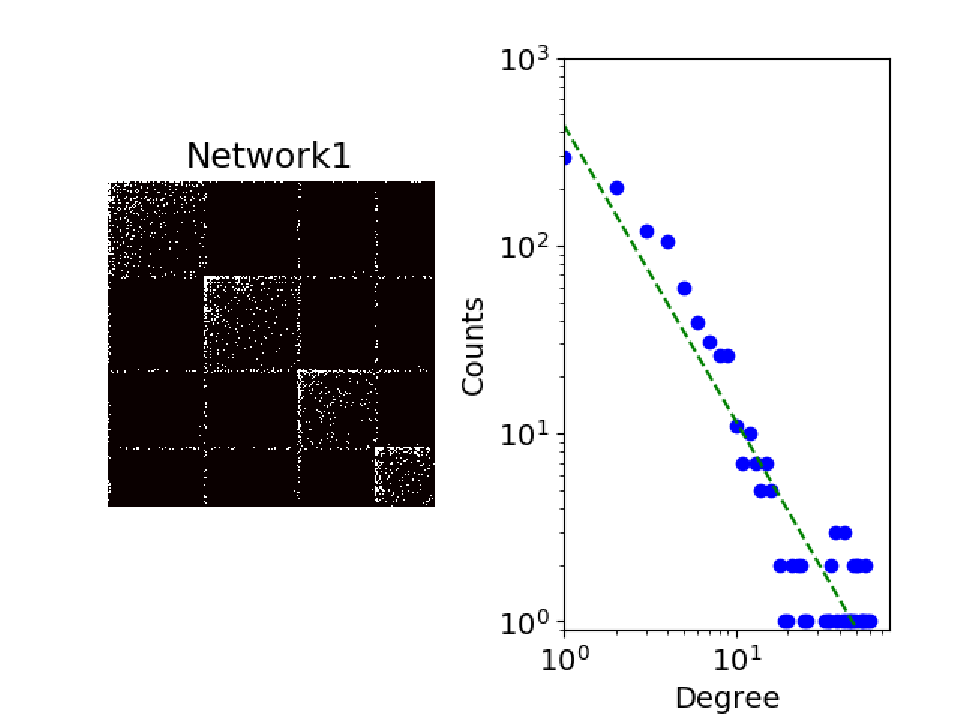
\includegraphics[width=\textwidth]{img/corpus/network1_dd}
        \end{minipage}
        \begin{minipage}{0.4\textwidth}
            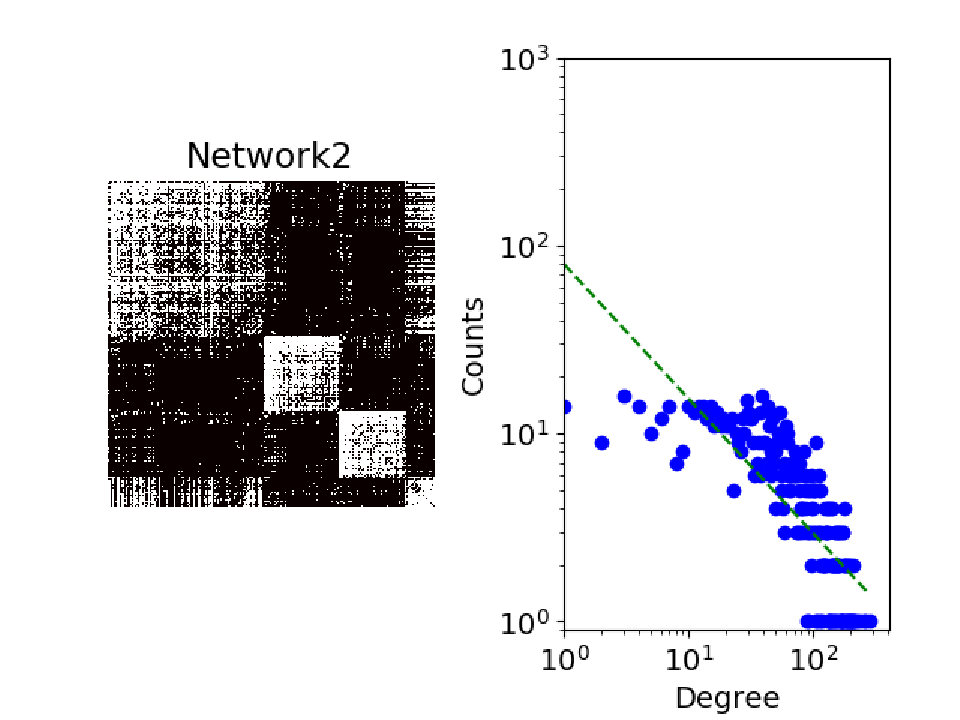
\includegraphics[width=\textwidth]{img/corpus/network2_dd}
        \end{minipage}
        %\vskip\baselineskip
        \begin{minipage}{0.4\textwidth}
            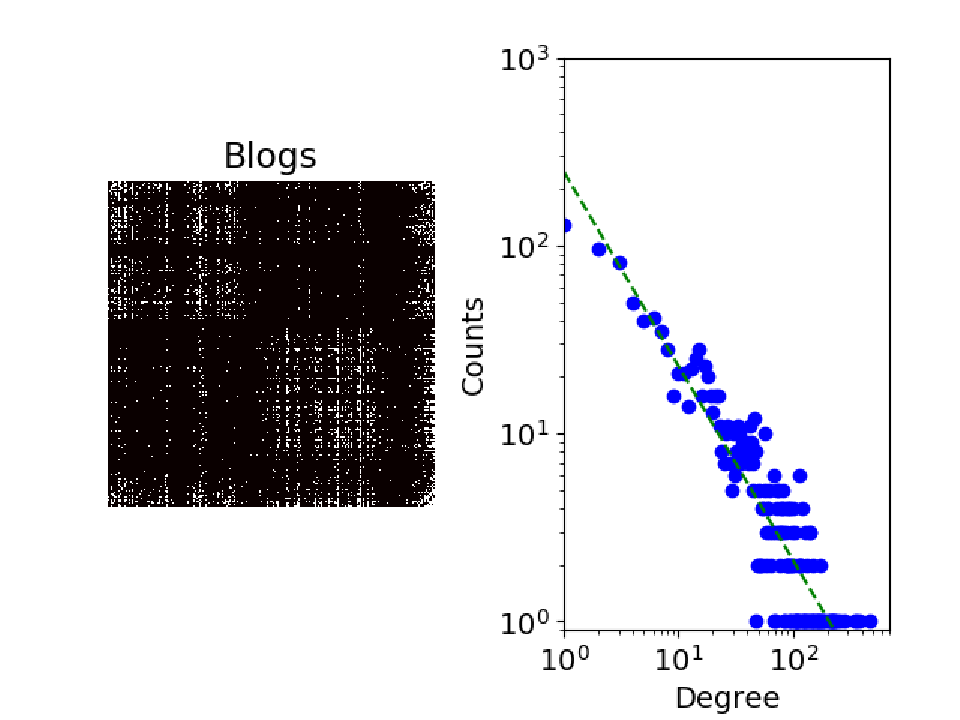
\includegraphics[width=\textwidth]{img/corpus/blogs_dd}
        \end{minipage}
        \begin{minipage}{0.4\textwidth}
            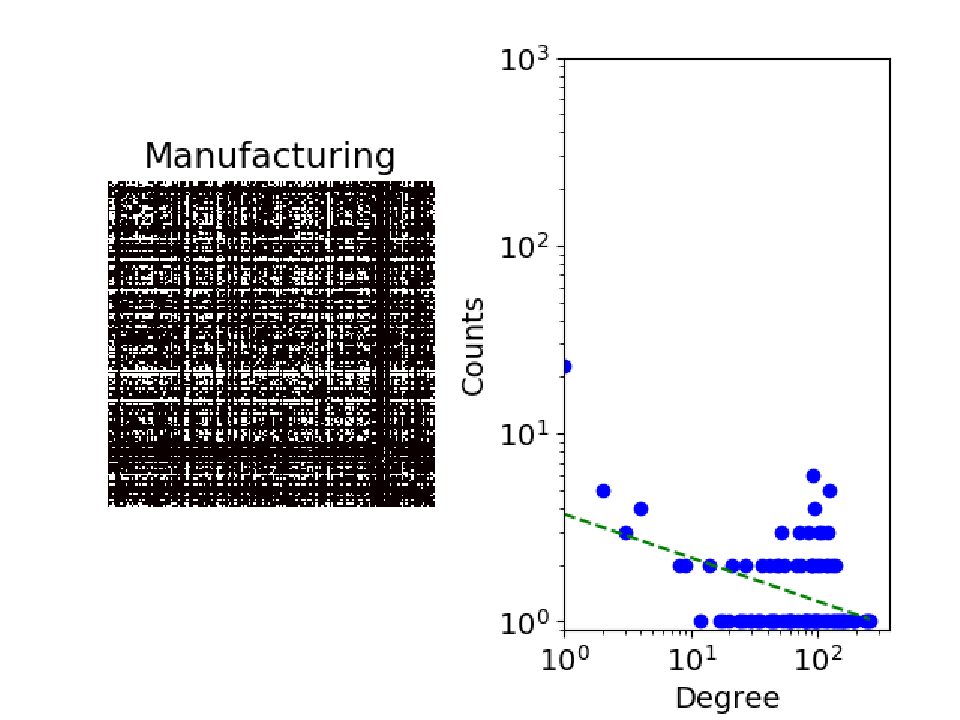
\includegraphics[width=\textwidth]{img/corpus/manufacturing_dd}
        \end{minipage}
	\caption{Adjacency matrices (left) and global degree distributions (right) for the four training datasets. In the adjacency matrices, a white dot corresponds to a 1 and a black dot to a 0.}
	\label{fig:corpuses}
\end{figure}

\begin{figure}[h]
    \centering
        \begin{minipage}{0.4\textwidth}
            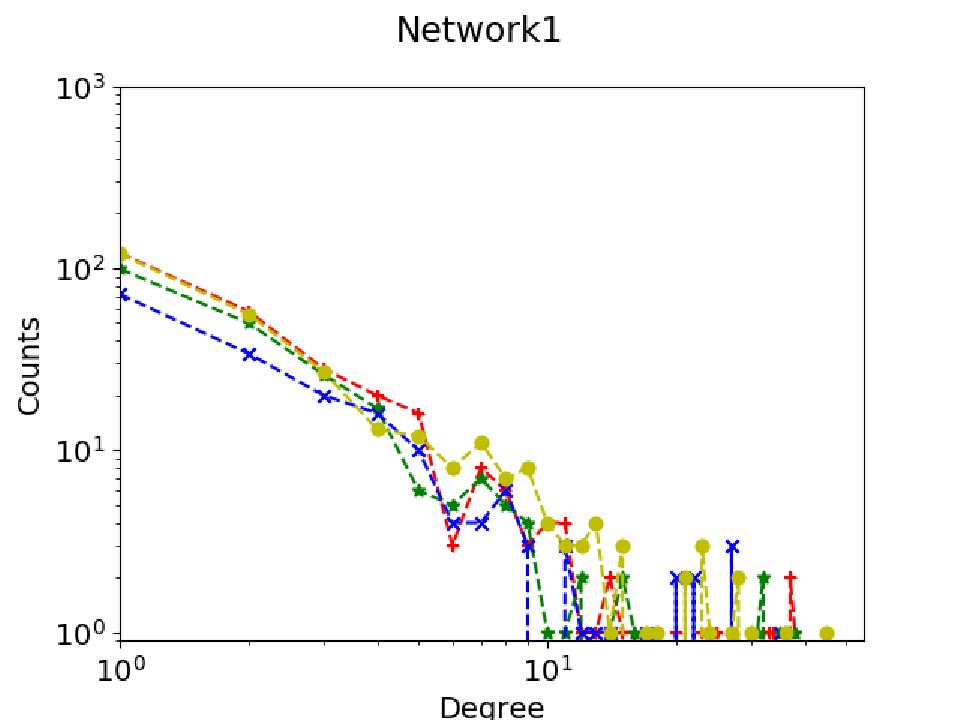
\includegraphics[width=\textwidth]{img/corpus/network1_1}
        \end{minipage}
        \begin{minipage}{0.4\textwidth}
            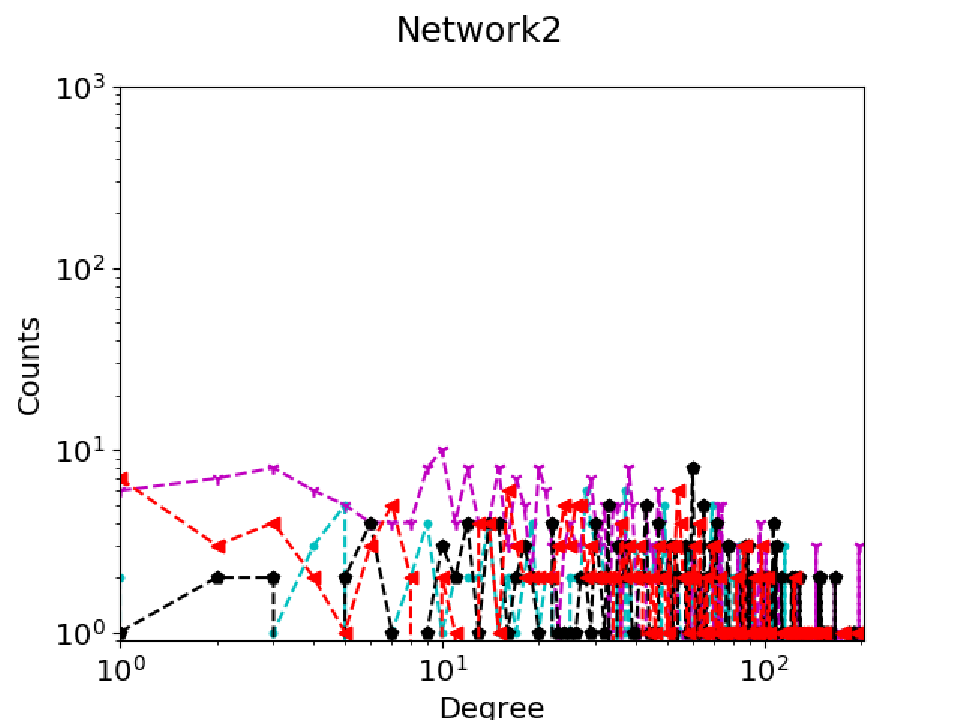
\includegraphics[width=\textwidth]{img/corpus/network2_1}
        \end{minipage}
        \vskip\baselineskip
        \begin{minipage}{0.4\textwidth}
            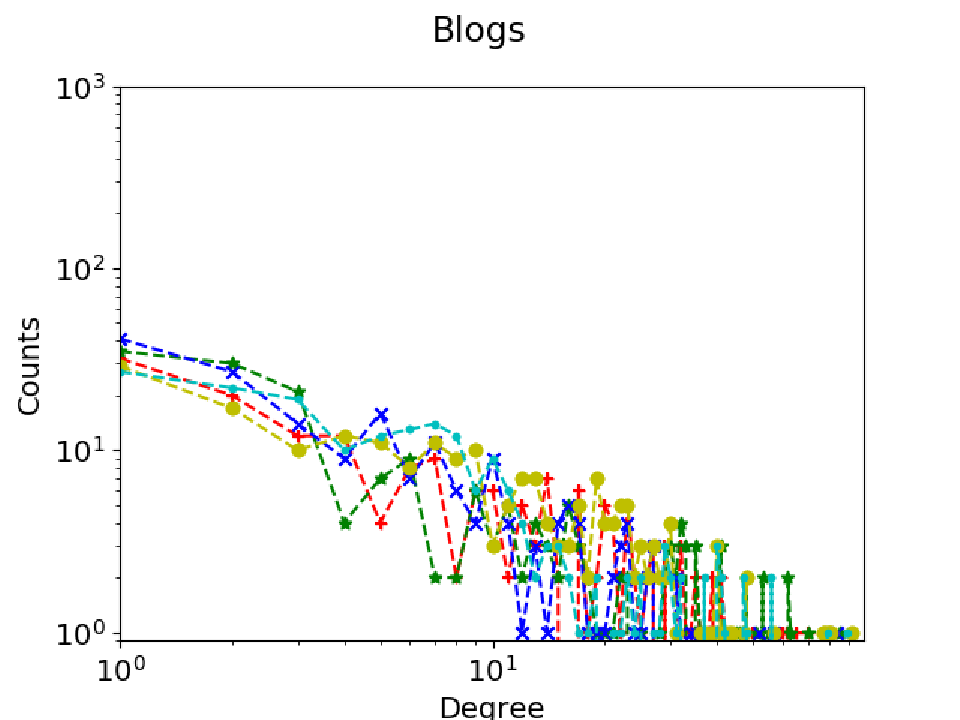
\includegraphics[width=\textwidth]{img/corpus/blogs_1}
        \end{minipage}
        \begin{minipage}{0.4\textwidth}
            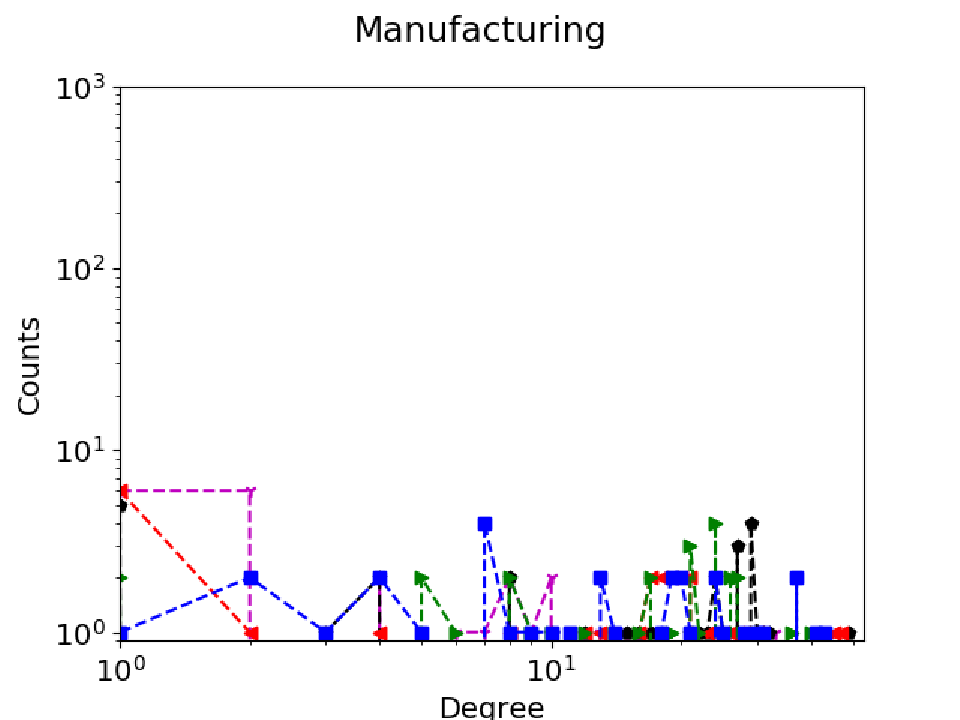
\includegraphics[width=\textwidth]{img/corpus/manufacturing_1}
        \end{minipage}
        \caption {Local degree distributions for the four training datasets. For Network1 and Network2 the classes come from ground-truth. For Blogs and Manufacturing, classes are obtained by Louvain algorithm.} 
	\label{fig:synt_graph_local}
\end{figure}

For each dataset, we estimate the model parameters through Markov Chain Monte Carlo inference consisting of 200 iterations. For \imb, the concentration parameters of HDP were optimized  using vague gamma priors $\alpha_0 \sim \text{Gamma}(1,1)$ and $\gamma \sim \text{Gamma}(1,1)$ following \cite{HDP}. The parameters for the matrix weights  $\lambda_0$ and $\lambda_1$ were fixed to 0.1. For \ifm, the hyperparameter  $\sigma_w$ was fixed to 1 and the IBP hyperparameter $\alpha$ to 0.5 in order to  have comparable number of classes with \imb. Once the models have been learned, they are used to generate links (or non-links) between the entire set of network nodes. The whole procedure is repeated 10 times and the average values are reported as final results.

\subsection{Homophily}

Figure \ref{fig:homo_mustach} presents boxplots describing the distributions of the natural $s_n(i,j)$ and latent $s_l(i,j)$ similarities computed respectively on linked and non-linked pairs of nodes for \imb\ (top) and \ifm\ (bottom). The results have been aggregated over the four datasets. They confirm that the natural similarity is  higher for pairs of nodes which are linked than for pairs of nodes which are not linked, for both models. For the latent similarity,  there is no difference between the linked and non-linked pairs, indicating that the links are not homophilic. These experimental results are in line with the theoretical results presented in Section~\ref{sec:homophily} that state that both \ifm\ and \imb\ are homophilic for  the natural similarity but are not homophilic for the latent similarity.

\begin{figure}[ht]
\centering
    \begin{subfigure}
       	 \centering
        	 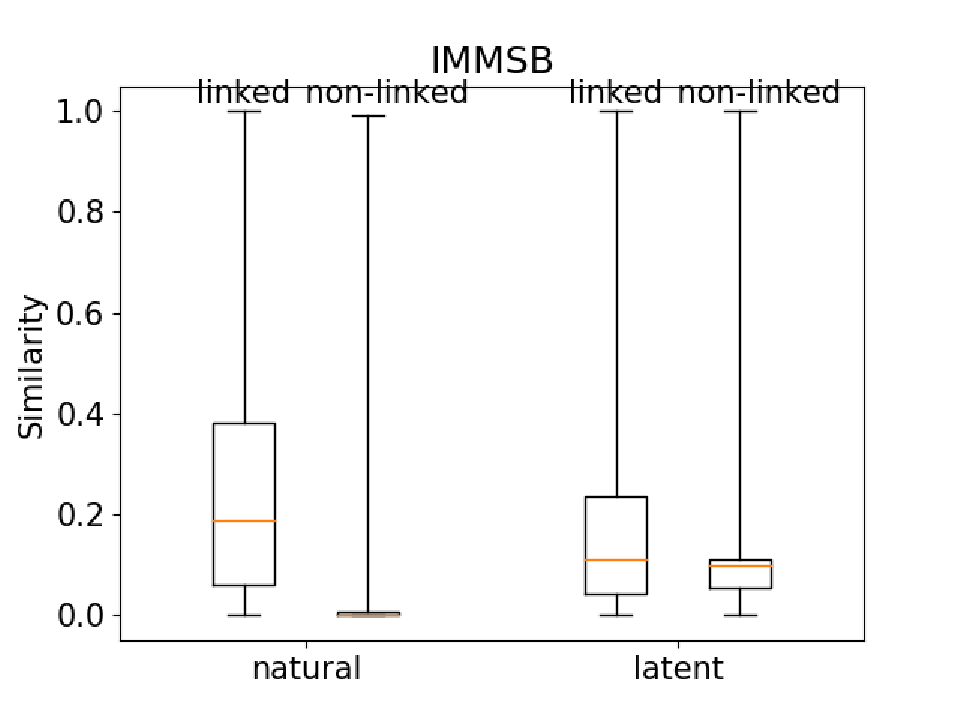
\includegraphics[width=0.38\textwidth]{img/corpus/homo_mustach_immsb}
    \end{subfigure}
    \begin{subfigure}
        	 \centering
          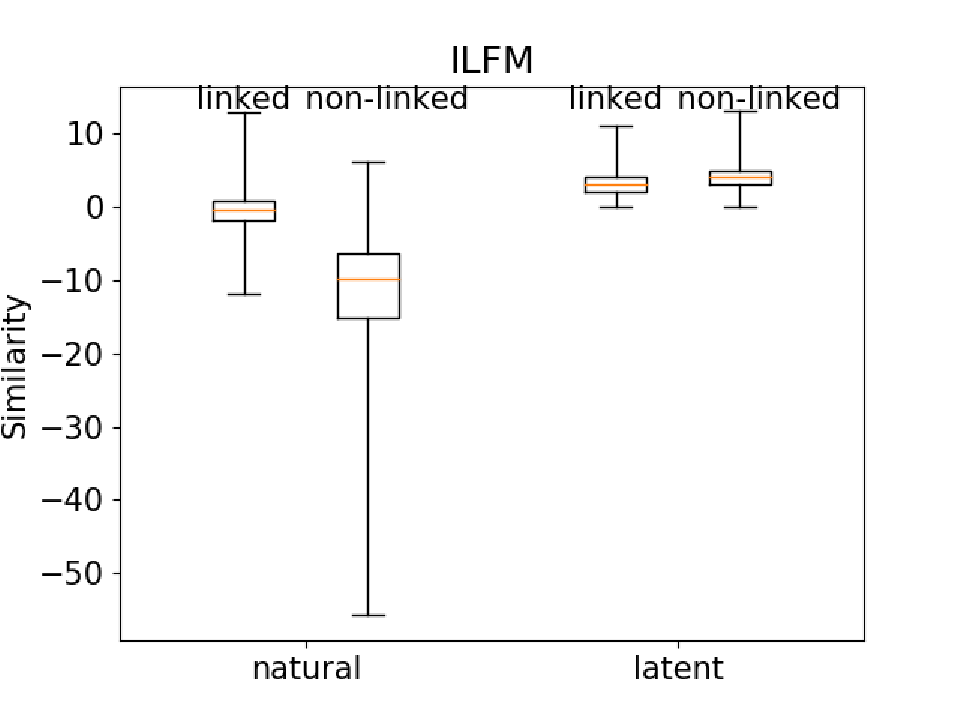
\includegraphics[width=0.38\textwidth]{img/corpus/homo_mustach_ilfm}
    \end{subfigure}
    \caption{Natural and latent similarities aggregated over all datasets and computed on linked and non-linked pairs of nodes for \imb\ (top) and \ifm\ (bottom).}
    \label{fig:homo_mustach}
\end{figure}

\subsection{Preferential attachment}

Table \ref{table:me_gofit} reports the value of the power-law goodness of fit for \imb\ and \ifm\ in the global case (left) and in the local case (right). It appears that for both models, the global preferential attachment is only verified for networks generated from datasets where the property was observed, namely in Network1 with p-value equal to 0.9 for \imb\ and 1 for \ifm, and in Blogs with a p-value equal to 1 for both models; the property is not verified in Network2 and in Manufacturing, where p-values are equal to 0. This is in accordance with Proposition 2.1 according to which both \ifm\ and \imb\ do not satisfy global preferential attachment. However, these models are able to capture this property if it exists in the training datasets.  Moreover, one can observe that, in the local case, \imb\ complies with the preferential attachment with $p$-values equal or close to 1 for the four networks, while \ifm\ obtained low p-values for the networks that were less locally bursty (respectively  0  for Network2 and 0.3 for Manufacturing). In addition, the power-law coefficients $\alpha$ are significantly greater for \imb\ than for \ifm, and specially for the bursty networks Network1 and Blogs.

Figure \ref{fig:me_local} illustrates the local preferential attachment for Network1 (top) and Network2 (bottom) estimated with \imb\ (left) and \ifm\ (right). The shape of the local degree distributions appears more linear for \imb\ and with more fluctuations for \ifm. This illustrates the fact that \ifm\ does not capture local preferential attachment whereas \imb\ does, as stated in Proposition 2.2. 


\begin{table}[h]{Preferential attachment measures for training datasets and networks generated with fitted models.}
\begin{tabular}{lrrrr}
  \multirow{2}{*}{\textbf{Training Datasets}}  &
  \multicolumn{2}{c}{Global} & \multicolumn{2}{c}{Local}\\
  \cmidrule(r){2-3} \cmidrule(l){4-5}
  &   $p$-value &   $\alpha$   & $p$-value & $\alpha$   \\
\hline
Network1       & 1 & 2.4 &   1.0 $\pm$ 0.0  &  1.8 $\pm$ 0.03  \\
Network2       & 0 & 1.3 &   0.0 $\pm$ 0.0  &  1.2 $\pm$ 0.01 \\
Blogs          & 1 & 1.5 &   1.0 $\pm$ 0.0  &  1.4 $\pm$ 0.03\\
Manufacturing  & 0 & 1.4 &   0.4 $\pm$ 0.3  &  1.3 $\pm$ 0.05 \\
\hline

  \ \textbf{\immsb} &&&& \\
\hline
Network1       & 0.9 & 1.4 &   1.0 \(\pm\) 0.0   &  3.5 \(\pm\) 0.7 \\
Network2       & 0 & 1.3 &   0.9 \(\pm\) 0.0   &  1.6 \(\pm\) 0.2 \\
Blogs          & 1 & 1.3 &   1.0 \(\pm\) 0.0   &  4.3 \(\pm\) 1.1 \\
Manufacturing  & 0 & 1.2 &   0.9 \(\pm\) 0.01  &  1.6 \(\pm\) 0.1 \\
\hline

  \ \textbf{\ilfm} &&&& \\
\hline
Network1      & 1 & 1.4 &   1.0 \(\pm\) 0.0  &  1.7 \(\pm\) 0.1 \\
Network2      & 0 & 1.2 &   0.0 \(\pm\) 0.0 &  1.2 \(\pm\) 0.0 \\
Blogs         & 1 & 1.3 &   0.9 \(\pm\) 0.2  &  1.5 \(\pm\) 0.1 \\
Manufacturing & 0 & 1.2 &   0.3 \(\pm\) 0.3  &  1.3 \(\pm\) 0.0 \\
\hline
\end{tabular}
\label{table:me_gofit}
\end{table}


\begin{figure}[h]
    \centering
    \begin{minipage}{0.4\textwidth}
        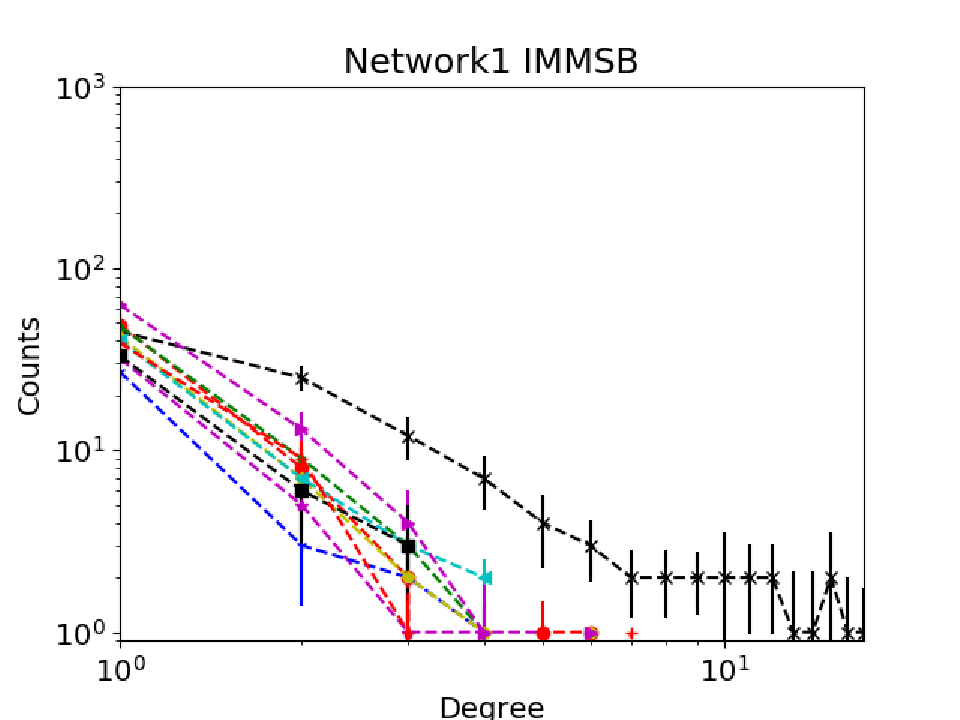
\includegraphics[width=\textwidth]{img/corpus/immsb_network1_1}
    \end{minipage}
    \begin{minipage}{0.4\textwidth}
        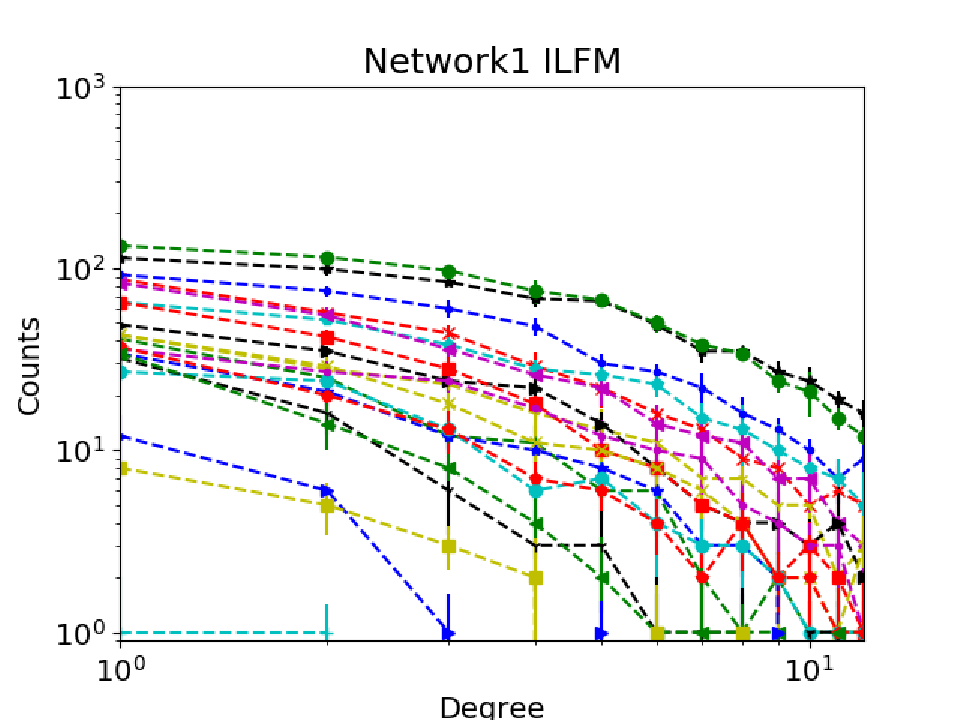
\includegraphics[width=\textwidth]{img/corpus/ilfm_network1_1}
    \end{minipage}
    \vskip\baselineskip
    \begin{minipage}{0.4\textwidth}
        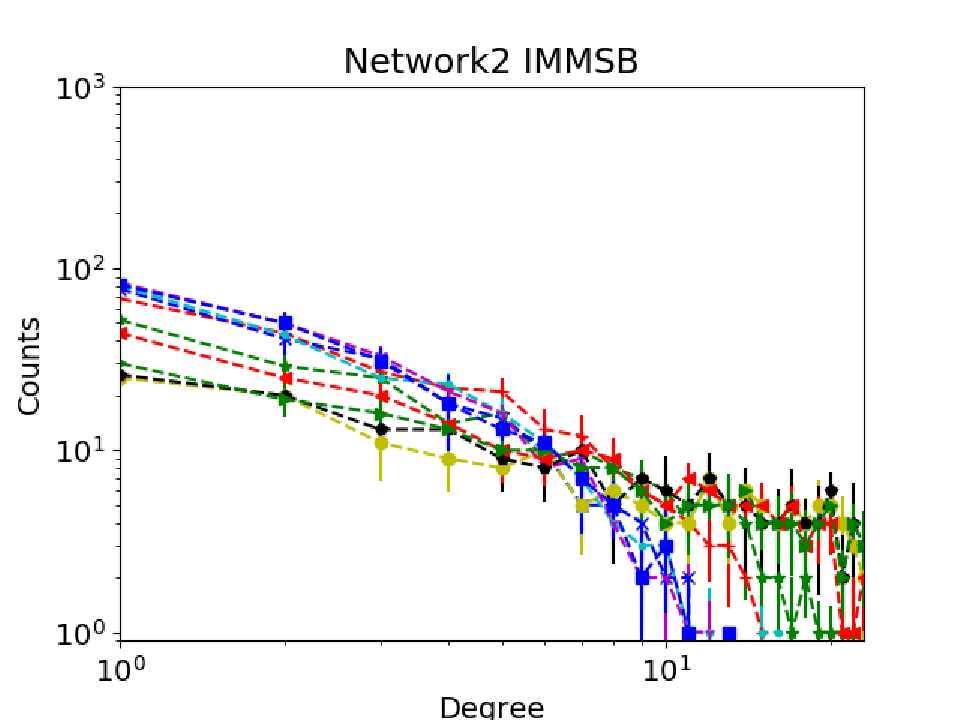
\includegraphics[width=\textwidth]{img/corpus/immsb_network2_1}
    \end{minipage}
    \begin{minipage}{0.4\textwidth}
        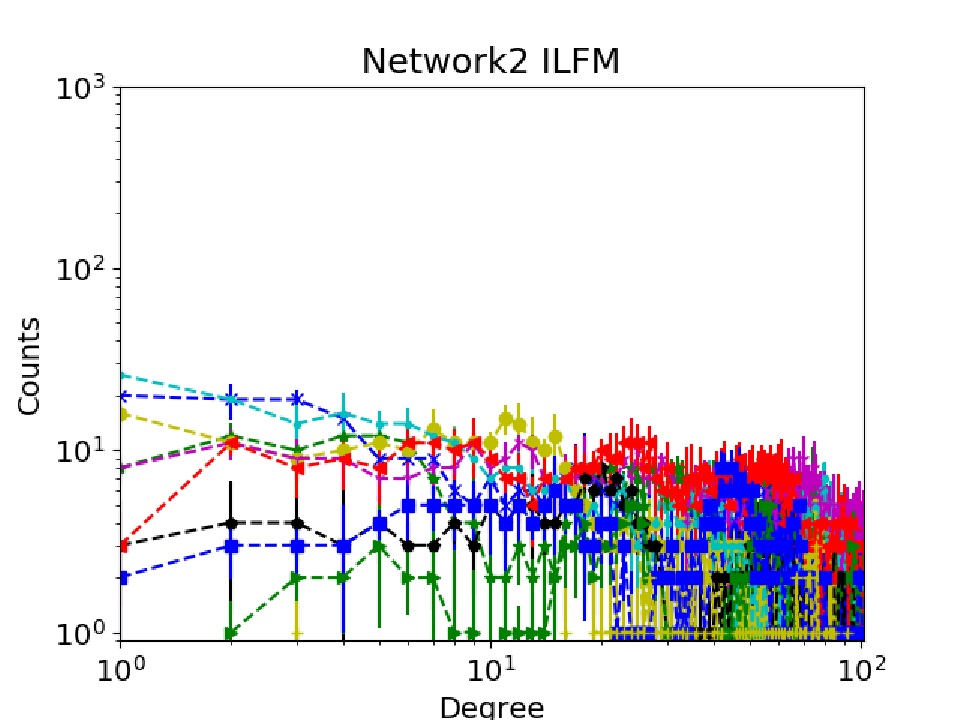
\includegraphics[width=\textwidth]{img/corpus/ilfm_network2_1}
    \end{minipage}
    \caption {Local degree distributions for Network1 (top row) and Network2 (bottom row) generated with fitted models \imb\ (first column) and \ifm\ (second column).} 
\label{fig:me_local}
\end{figure}

\begin{figure}[ht!]
\centering
    \begin{minipage}{0.4\textwidth}
        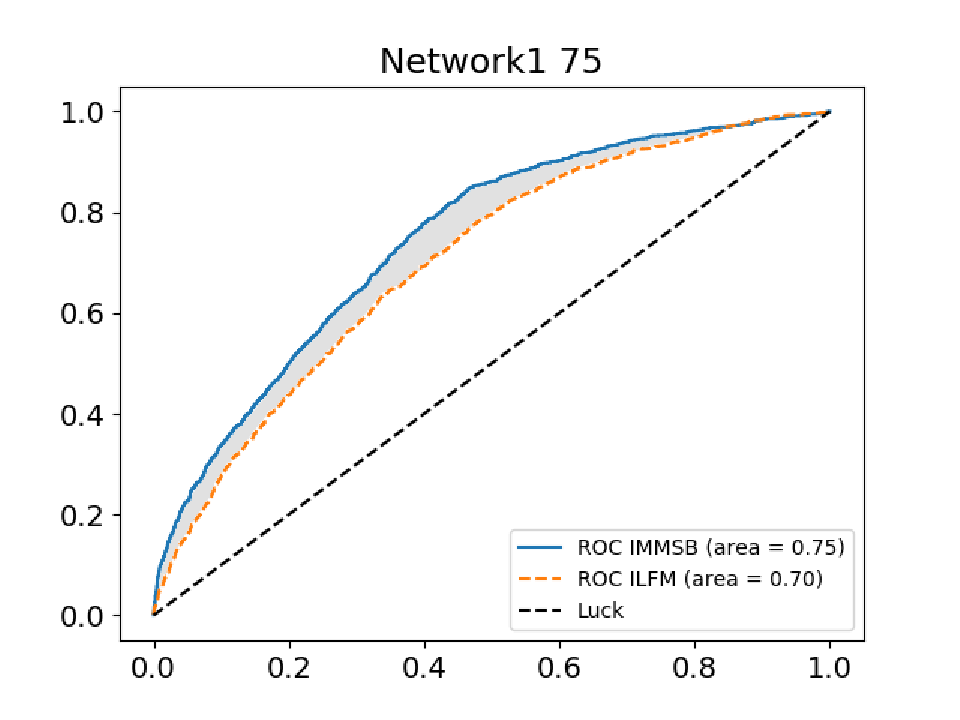
\includegraphics[width=\textwidth]{img/corpus/roc_network1_75_f}
    \end{minipage}
    \begin{minipage}{0.4\textwidth}
        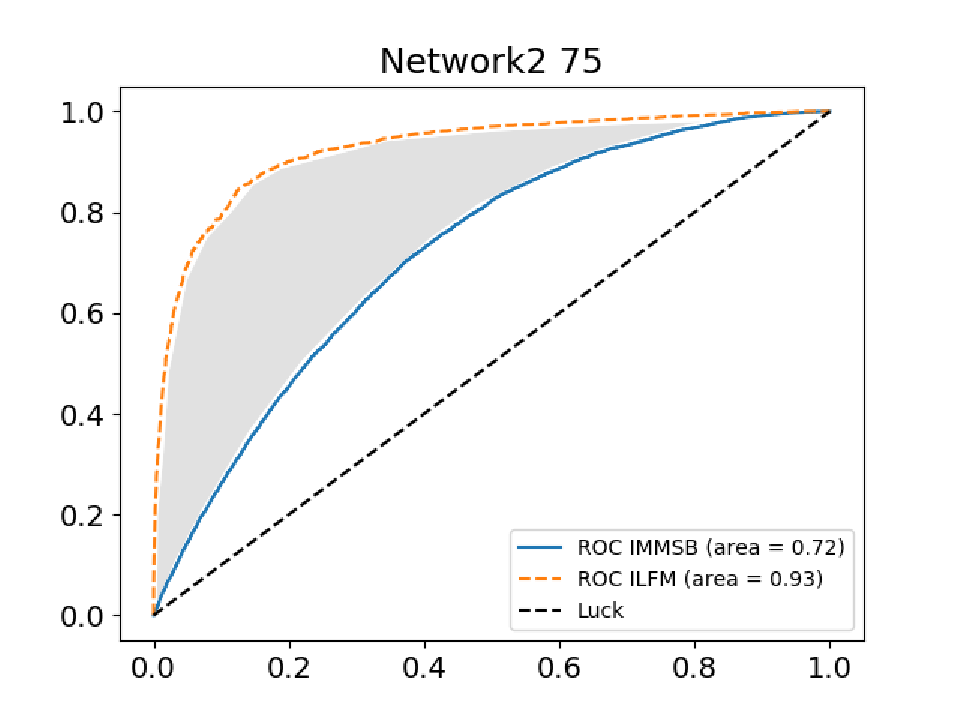
\includegraphics[width=\textwidth]{img/corpus/roc_network2_75_f}
    \end{minipage}
    \begin{minipage}{0.5\textwidth}
        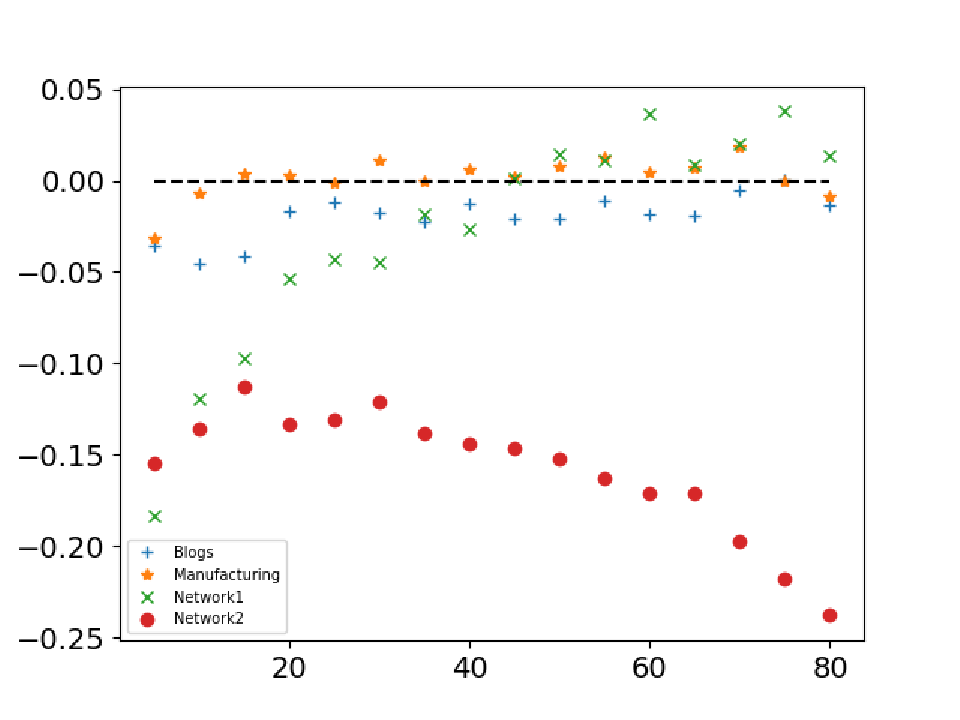
\includegraphics[width=\textwidth]{img/corpus/testset_max_20}
    \end{minipage}
    \caption{Top: AUC-ROC curves for Network1 (left) and Network2 (right) with 75 percent of data used for learning that compares the performance of models. Bottom: Relative performance of \imb\ and \ifm\ according to the percentage of data used for testing, the rest being used for learning.} 
\label{fig:auc}
\end{figure}

Lastly, Figure \ref{fig:auc} compares the performance of the models for predicting new links using the Area Under the Curve (AUC) measure as a function of the training set size. In the bottom plot, the y-axis gives the relative performance defined as the difference of the AUC values for \imb\ and \ifm\ ($AUC_{\imb} - AUC_{\ifm}$) whereas the x-axis indicates the percentage of links randomly removed from the datasets and used as test examples. Hence, the number of training data decreases with the x-axis and a positive value on the y-axis indicates that \imb\ outperforms \ifm.  The relative performance corresponds to the difference of the MAX AUC values obtained for both models on the 10 inference experiences. The top plots illustrate a case where 75 percent of the data is used as test set and where \imb\ dominates \ifm\ on Network1 (left), and the opposite on Network2 (right).

In general, as shown in the bottom plot, \ifm\ obtains better performance than \imb. However, the relative predictive performance of \imb\  increases  when the quantity of training data decreases on bursty networks, whereas for non-bursty networks the results are the opposite: the performance of \ifm\ increases when the size of the learning dataset decreases. This is particularly visible for Network2. The results for Manufacturing are less marked, which is certainly due to the small size of this network, making the prediction less challenging.

The above behavior can be explained by the fact that \imb\ satisfies the local preferential attachment whereas \ifm\ does not: as links are randomly removed, one is more likely to remove links from large classes than from small ones; a model that enforces local preferential attachment on bursty networks is thus more likely to reconstruct those removed links. This is what is happening on Network1 and Blogs for \imb. On the contrary, for non-bursty networks, a model enforcing local preferential attachment is penalized.

%\section{Generative Context -- $M_g$}
%    
\subsection{Preferential Attachments: Extensions and generalization}

In this section we provide an extension of the study of the preferential attachment in two directions :
\begin{itemize}
    \item Recall the representation theorem \cite{orbanz2015bayesian} about exchangeable sequence and arrays and it's consequences on random networks.%Show the relation between exchangeable sequence (jointly exchangeable adjacency matrix) and the burstiness phenomenon associated to the sum over realization of the exchangeable sequence,
    \item Characterizing the burstiness phenomenon over the size of the classes that the models produce in their generative process (feature burstiness). 
    \item Specifying the limitation of studying the preferential attachment in the $me$ context by specifying it's relation with $mg$. The $mg$ context represents the models seen from it's hyper-parameters while $me = (\hat F, \hat \Phi)$ represents the model seen from an estimated model (with a inference procedure like a MCMC or a variational inference).
\end{itemize}

\subsubsection{Recall of Definitions and Theorems on Exchangeability}~\\

An exchangeable sequence is a sequence $X := (X_1 \in A_1, X_2 \in A_2,...)$ of random variables whose joint distribution satisfies :
\begin{equation}\label{eq:exch}
P(X_1 \in A_1, X_2 \in A_2,...) = P(X_{\pi(1)} \in A_1, X_{\pi(2)} \in A_2,...)
\end{equation}

for every permutation $\pi$  of integers and collection $A_1, A_2,...$ of measurable sets. Following the notation in \cite{orbanz2015bayesian} we can express \eqref{eq:exch} by $P(X_n) = P(X_{\pi(n)})$. In order to characterize the adjacency matrix underlying a social network, we can extend the definition of sequence by denoting a random matrix as $(X_{ij})_{i,j \in \mathbb{N}}$. Thus we says that the random matrix $X$ is jointly exchangeable if it satisfies :
	\begin{equation}
	P(X_{ij}) = P(X_{\pi(i)\pi(j)})
	\end{equation}
	
The Aldous-Hoover theorem generalizes the representation theorem for exchangeable sequence of De-Finetti for exchangeable matrix. It states that a random matrix $(X_{ij})$ is a jointly exchangeable matrix if and only if it can be represented as follows : There is a random measurable function $F:[0,1]^3 \rightarrow X$ such that : 
\begin{equation}
X_{ij} \sim F(U_i, U_j, U_{\{\{i,j\}\}})
\end{equation}

where $(U_i)_{i\in \mathbb(N)}$ and $(U_{\{\{i,j\}\}})_{i, j\in \mathbb(N)}$ are, respectively, a sequence and matrix of i.i.d. Uniform[0,1] random variables.

A important consequence of the Aldous-Hoover theorem is that an exchangeable graph is either empty or dense. It means that if the graph is not empty, the number of edges $n$ will be lower bounded by $cn^2$ with $c$ a constant. This  come from the the fact that edge proportion is independent of $N$ and can be computed as follows $\epsilon = \int_{[0,1]^3} F(x, y, z)dxdydz$.

~\\
We illustrate this results for (i)MMSB model (for the nonparametric version, note that the support of $k$, and $\bm\alpha$ is theoretically infinite and in the latter drawn from a stick breaking process  $\bm \alpha \sim SB(\gamma)$), by marginalizing over the model parameters, we can compute the expected proportion of edges in the graph $G$ :

\begin{align*}
&p(y_{ij}=1| \bm{\alpha}, \bm{\lambda}) = \int_{f_i} \int_{f_j} \int_{\Phi} p(f_i| \alpha ) p(f_j| \alpha)p(\Phi| \lambda) \\
&\times \sum_{k,k'} p(y_{ij} \mid \phi_{kk'})\ p(k\mid f_i)p(k'\mid f_j)df_i df_j d\Phi \\
&=  \sum_{k,k'} \int_{\Phi} \phi_{kk'} p(\Phi| \lambda) d\Phi \int_{f_i} f_{ik} p(f_i| \alpha )df_i \int_{f_j} f_{jk}  p(f_j| \alpha ) df_j \\
&= \sum_{k,k'} \E[B(\lambda_1, \lambda_0)] \E_k[Dir(\mat{\alpha} )] \E_{k'}[Dir(\mat{\alpha})] \\
&= \frac{\lambda_1}{\lambda_0+\lambda_1}\frac{\sum_{k,k'} \alpha_k\alpha_k'}{(\sum_k \alpha_k)^2} = \epsilon
\end{align*}

It follows that this expectation do not depend on the number of vertex $n$, and the expected number of edges for an undirected graph is $\dbinom{n}{2} \epsilon = O(n^2)$.

Note that for ILFM, the expected proportion of edges in the graph don't take a closed form expression since the (kernel) likelihood is not conjugate with the Indian Buffet Process :

\begin{equation}
P(y_{ij}=1 | \alpha, \sigma) = \int_\Phi \sum_F p(y_{ij}=1 | \Phi, F)P(F | \alpha) P(\Phi|\sigma) d\Phi
\end{equation}

There is no closed form for this expression due to it's non-conjugacy.

Here is the different component of this previous equation for completeness \cite{IBP} :
\begin{equation}
p(y_{ij}=1 | \Phi, F) = \sigma(f_i\Phi f_j^T)
\end{equation}

\begin{equation}
p(\Phi|\sigma) = \prod_{k, k'} P(\phi_{k,k'}|\sigma) \qquad \mathrm{with} \quad P(\phi_{k,k'}|\sigma) = N(0, \sigma)
\end{equation}

\begin{equation}
P(F \mid \alpha) = \frac{\alpha^{K_+}}{\prod_{i=1}^N K_1^{(i)} } \exp(-\alpha H_N) \prod_{k=1}^{K_+} \frac{(N - m_k)!(m_k - 1)!}{N!}
\end{equation}

Where $H_N = \sum_{j=1}^N \frac{1}{j}$ is the Nth harmonic number, $m_k$ the number of observations containing feature $k$ and $K_+=K-K_0$ is the number of represented features where $K_0$ is the number of observation for which $m_k=0$.



\subsubsection{Feature burstiness}~\\

We propose a third definition for the study of the preferential attachment in social networks. It concerns the preference that an individuals would have to join a class given the current number of actual members. Thus the quantity we study here correspond to the size of the classes : thus we add the following third definition to the previous section : 

To pursue this definition, one need to precise what precisely means the "size of a class". Depending on what is the definition of the membership within a class that we consider, the notion of size will differs.

We consider the two following cases, which defined the relative size $N_k^i$ for any node $i$. It represents the size of class from a node point a view and can be interpreted as the potential number of nodes that a given node $i$ can bind to :
\begin{itemize}
    \item Soft membership - IMMSB : In this case, nodes belongs to every classes in different proportion. The size of class refers in this case to the number of relation (linked or non-linked) within a class who depends on the random tensor $Z$ : $N_k^i = \sum_{j \in V} \delta(z_{i\rightarrow j}=k)\delta(z_{j\rightarrow i}=k)$,
    \item Hard membership - ILFM : This case correspond to the number of nodes falling joitly in a class since the membership is in the binary set \{ \emph{belongs} or \emph{not belongs} \}, which depends on the random matrix $F$ : $N_k^i = \sum_{j\in V} f_{ik}f_{jk}$.
\end{itemize}

From that definition, one can compute the size of a class as $N_k = \sum_{i\in V} N_k^i$ and the following upper bounds hold for an undirected network model with self loop: $N_k^i \leq N$ and $N_k \leq \dbinom{N}{2}$.

The question that arise is how are distributed the $N_{1:k}$ random variables and what is their bursty dynamic.

\begin{definition}[Preferential attachment (for class size)]
Let $k$ be a class in a social network and let $N_k$ denote its size. 
\begin{description}
    \item[(3)] \emph{feature preferential attachment}: we say that a probabilistic link prediction model $mg$ satisfies the feature preferential attachment iff, for any latent class $k$, the model satisfy the following , $\pr(N_k \ge n+1 \mid N_k \ge n, \mathcal{M}_g)$ increases with $n \in [0,\dbinom{N}{2}]$.
\end{description}
\label{def:burst-soc-net2}
\end{definition}


\begin{proposition}
Both ILFM and IMMSB respect the feature preferential attachment (with regularities conditions on hyperparameters for IMMSB).	
\end{proposition}

\begin{proof}[sketch]
	
For ILFM:

From node exchangeability on can write :
\begin{equation} \label{eq:feat_ex}
P(N_k=n) = \dbinom{N}{n}P(f_{1k}=1,..,f_{nk}=1,f_{(n+1)k}=0,..,f_{Nk}=0)
\end{equation}

It follows from the burstiness definition and Bayes' rule :
\begin{equation}
\frac{P(N_k=n+1)}{P(N_k=n)} = \frac{N-n}{n+1}P(f_{ik}=1 | F_{.k}^{-ik})
\end{equation} 

Here, the node index $i$ is a free variable since the sequence in equation \eqref{eq:feat_ex} is exchangeable, who can choose any nodes.

As $F$ is drawn from an Indian Buffet Process, we have $P(f_{ik}=1 | F_{.k}^{-i}) = \frac{n}{N}$.\\


For IMMSB: 

Remark: note if $N_k^i$ is bursty, it implies that $N_k$ is also busrty from its definition because the sum conserve the inequality. And in the former case the burstiness is then stronger than the second.

From the node exchangeability, one can write :

\begin{align*}
P(N_k^i=n) &= \dbinom{N}{n}P(z_{i\rightarrow 1}=k,z_{i\leftarrow 1}=k,..,z_{i\rightarrow n}=k, z_{i\leftarrow n}=k, \\
 &z_{i\rightarrow n+1}\neq k, z_{i\leftarrow n}\neq k,..,  z_{i\rightarrow N}\neq k, z_{i\leftarrow N}\neq k)
\end{align*}

Again, it follows from the burstiness definition and Bayes' rule :
\begin{equation} \label{eq:memb_ex}
\frac{P(N_k^i=n+1)}{P(N_k^i=n)} = \frac{N-n}{n+1}P(z_{i\rightarrow j}=k,z_{i\leftarrow j}=k | Z_{i\rightarrow}^{-j}, Z_{i\leftarrow}^{-j})	
\end{equation}

The right part of equation \eqref{eq:memb_ex} has known closed form similar to the collaped Gibbs update for the membership assignment of IMMSB (see annexe). The burstiness equation reduce to :

\begin{align*}
\frac{P(N_k^i=n+1)}{P(N_k^i=n)} &= \frac{N-n}{n+1}P(z_{i\rightarrow j}=k | Z_{i\rightarrow}^{-j},) P(z_{i\leftarrow j}=k |  Z_{i\leftarrow}^{-j}) \\
&=  \frac{N-n}{n+1} \left( \frac{n + \alpha_k}{N + \alpha_{\bm{.}}}\right)^2
\end{align*}

\textcolor{red}{Here, there is this polynom of order 2 to solve to find the constraint on $\alpha$ to satisfy the burstiness, I skip it to win some times for now...}

\end{proof}


\subsubsection{Local preferential attachment - General case}~\\

In the previous part we studied the preferential attachment in a context where we fit the model parameters. We showed that according to the type of prior (hard vs soft), it impacted the preferential attachment properties on the random network. To highlight this property we only needed to focus our analysis on the distribution conditioned on what we called $me$, which is actually an estimation of the parameters $F$ and $\Phi$ noted $\hat F$ and $\hat \Phi$. Those learned parameters are drawn from an approximate posterior noted $\hat P(F, \phi | Y, mg) \propto P(Y|F, \Phi)P(F|mg)P(F|mg)$ which came from the inference process such that $me = (\hat F, \hat \Phi) \sim \hat P(F, \phi | Y, mg)$. Thus which approximates the true posterior and provide the following generative equations :

\begin{equation}
    p(Y | \hat F, \hat \Phi) = \prod_{i<j} f_i \Phi f_j^T
\end{equation}

We define the expected degree as :

\begin{equation}
d_{i}^{mg} = \sum_{j\in V} p(y_{ij}=1 | mg)
\end{equation}

It is straightforward that the expected (global) degree is constant for any nodes in the networks for exchangeable models since  the expected link prediction is constant with $N$, and so on for IMMSB and ILFM. 

Nevertheless one can ask about the  expected (local) degree inside a class. The expected local degrees ($mg$ case) given a class, is trivially given from the graphical models and correspond the following quantities  :
\begin{itemize}
	\item $\sum_{j\in V} p(y_{ij}=1  | z_{ij, ij}=k, mg) = N \lambda_1 / (\lambda_1 + \lambda_0)$ for IMMSB,
	\item $\sum_{j\in V} p(y_{ij}=1  | f_{ik, jk}=1, mg)$  for ILFM. Note that we can't compute it in a closed form expression for the same reason that previously of non-conjugacy.
\end{itemize}

In the general case, if we don't know the class a priori, the local degree expectation take the following form :

\begin{itemize}
\item  $d_{i,k}^{mg} = \sum_{j\in V} p(y_{ij}=1, z_{ij, ij}=k | mg)$ for IMMSB,
\item  $d_{i,k}^{mg} = \sum_{j\in V} p(y_{ij}=1, f_{ik, jk}=1| mg)$ for ILFM.
\end{itemize}

Note that it is easy to show we use this definition to define the degree in the $me$ context :
\begin{align*}
 d_{i,k}^{me} &= \sum_{j\in V} p(y_{ij}=1, z{i\rightarrow j}=k, z_{i\leftarrow j =k} | me) \\
  &= L(\phi_{kk} f_{ik} f{jk})
 \end{align*}
 
With the function $L()$ being the sigmoid for ILFM and the identity for IMMSB.

In turns out that again, this expected local degree have a closed form for (i)MMSB, and not for ILFM. For IMMSB we have the following :

\begin{align*}
p(y_{ij}=1, z_{ij, ij}=k | mg) &= p(y_{ij}=1 |  z_{ij, ij}=k, mg) p( z_{ij, ij}=k | mg) \\
 &=E_{\phi_{kk}}[ p(y_{ij}=1 |  z_{ij, ij}=k, \phi_{kk}, mg) ] E_{f_i}[ p( z_{ij}=k | f_i, mg)] E_{f_j}[ p( z_{ji}=k | f_j, mg)] \\
 &= \frac{\lambda_1}{\lambda_0+\lambda_1}\frac{ \alpha_k\alpha_k'}{ (\sum_k \alpha_k)^2}
\end{align*}

Note that from our definitions we have $d_i^{mg} = \sum_k d_{i,k}^{mg}$.


\paragraph{}
\textcolor{red}{Remark on the definition of the burstiness in the $mg$ mode (expected degree):
\hrulefill
\hrulefill
~\\
}

for the burstiness in the "$mg$" with de degree local defined as $d_{i,k}^{mg}$  is trivially bursty, but makes no so much sense for the following reason :

The burstiness equation in this context can be written as :

\begin{equation}
b_n = \frac{p(d_{i,k}^{mg} = n+1)}{p(d_{i,k}^{mg} = n)}  \nearrow_? n 
\end{equation}

We know that $d_{i,k}^{mg} = N \epsilon_k$ which is equivalent to says that $p(d_{i,k}^{mg})$ is a Dirac distribution noted $\delta (N\epsilon_k)$. It means that the burstiness equation is only definite for $n = N\epsilon_k$, (otherwise the denominator is null), and hence its derivative is not defined.


\textcolor{red}{End fo Remark
\hrulefill
\hrulefill
~\\
}

The question of the local burstiness we should ask instead, is by seeking what are the sequence that underly a random variable that we want to analyze Here $d_{i,k}$ should not been seen as the sum over independent marginal probability, but as the joint probability of every draw concerned. 

In a first approach, let's assume we know the relative size of the class $k$ noted $N_i^k$:

\begin{align*}
P(d_{i,k}=n | mg) &= \dbinom{N}{n} P(\{y_{ij}=1, z_{\{ij,ji\}}=k, j\in [1,n]\}, \\ & \{y_{ij}=0, z_{\{ij,ji\}}=k, j\in [1,N_i^k-n]\}, \\
&  \{\ z_{\{ij,ji\}}\neq k, j\in [1,N-N_i^k]\}) \\
\end{align*}


\textcolor{red}{Iam not sure about the number of combination here, I need to think about it.}
 % burtisness only
%    
\subsection{Illustration}

todoso

%
\section{Conclusion}
\label{sec:concl}

We have studied whether stochastic mixed membership models, such as \ifm\ and \imb\, can generate new links while satisfying properties frequently verified in real  social networks, namely homophily and preferential attachment. To do so, we have introduced formal definitions of these properties and have analyzed how these models behave according to those definitions. We have shown, in particular, that both models are \textit{homophilic} with the natural similarity that underlies them. Concerning preferential attachment, we have shown that stochastic mixed membership models do not comply with global preferential attachment. The situation is however more contrasted when the property is considered at the local level: \imb\ enforces local preferential attachment whereas \ifm\ does not.~\\

These findings have been validated experimentally on two real and two artificial networks that have different degrees of global and local preferential attachment. An important, practical finding of our study is that \imb, usually considered of lesser "quality" than \ifm, can indeed yield better results on bursty networks (\textit{i.e.} networks with preferential attachment) when the number of training data is limited.~\\

There are many directions to extend this work with the motivation of improving our theoretical understanding of graphical models for link prediction in complex networks. A straightforward extension is to examine the relation between the local preferential attachment and the dynamic of the latent classes.  
%For example, some special value of the hyperparameters, of the non-parametric priors, could lead to a very large number of classes or, at the opposite, just one class. Between these two extremes, that goes from a vanishing local aspect of the degree distribution to a number of classes that overfit the data, on can ask how this parameter affect the global and the local degree distribution of a random graph.  
For instance, a fundamental result is the Aldous-Hoover theorem, which implies that exchangeable random graphs cannot be sparse \cite{orbanz2015bayesian}. It seems that the sparsity is related in some way to the preferential attachment in a network. Thus, the following question arises: would it be realistic to assume the exchangeability hypothesis for the local case but not for the global case, and how this fact impacts the burstiness of the global degree distribution and the sparsity of the graph.

We believe that answering to those questions open a way to develop and design Bayesian models able to better capture the fundamental properties of  real social networks.


~\\


\bibliographystyle{chicago}
%\bibliographystyle{unsrt}
\bibliography{./a}

\appendix
\section{Appendix}
\label{sec:append}

\subsection{Mixed membership Models}
\label{sec:mixmembership}
In the Mixed Membership Models \cite{MMM}, the models can be defined at the link level by the likelihood of generating a link between two nodes given the contribution of each classes (or features). For IMMSB, this likelihood is straightforward, but for ILFM the class membership is defined deterministically by the binary vector $\mat{f}$. If the $k^{th}$ row is active (equal to one) then the node has the membership, else it doesn't. Hence for ILFM, We can write the likelihood  using the Dirac distribution $\delta(x)$ that gives one for $x=0$ as follows:

\begin{align}
    \pr(y_{ij} \mid \mat{F}, \mat{\Phi } ) &= \sigma \sum_{k, k'} \pr(y_{ij}\mid\phi_{k,k'}) \pr(k \mid \mat{f}_i) \pr(k' \mid \mat{f}_j) \\
    &=  \sigma \sum_{k, k'} \phi_{k,k'}  \delta(1-f_{ik}) \delta(1-f_{jk'})
    \end{align}
    

\subsection{Collapsed Gibbs sampling updates for IMMSB}

We provide here the derivation of the updates of the IMMSB model, described in Section~\ref{sec:models}.

%From the definition of the model, one has: $\pr(z_{ij} = k \mid \mat{f}_i) = f_{ik}$.

%\textcolor{red}{Adrien, peux-tu donner la d\'erivation ? La forme actuelle n'est valable que pour MMSB.} 

%heeeere \alpha is \alpha_0

Inference for the IMMSB model by using the Collapse Gibbs sampler gives updates for class assignment $Z \in N\times N \times 2$ for each interactions $Y \in N\times N$. Thus for all pair of interaction (i,j) we jointly sample the classes $(z_{ij}, z_{ji})$ who implicitly, take the values $(k,k')$ :
\begin{align} \label{eq:cgs}
&\pr(z_{ij}, z_{ji} \mid Z^-, Y,  \mat{\beta}, \alpha, \mat{\lambda} )  \\
&\propto\pr(z_{ij}, z_{ji} \mid Z^-, \alpha,\mat{\beta}) \pr(y_{ij} \mid Y^{-ij},  Z^-,z_{ij}, z_{ji},  \mat{\lambda} ) \nonumber
\end{align}
The term $Z^-$ denote that both $z_{ij}$ and $z_{ji}$ are exclude from $Z$. We now treat the first term of equation \ref{eq:cgs}.  
\begin{align}
& \pr(z_{ij}, z_{ji} \mid Z^-, \alpha,\mat{\beta})\\
&\propto \pr(z_{ij} \mid \mat{z}_i^{-j}, \mat{z}_j, \alpha,\mat{\beta})  \pr(z_{ji} \mid \mat{z}_j^{-i}, \mat{z}_i, \alpha,\mat{\beta}) \nonumber
\end{align}
Let's consider the density of $z_{ij}$:
\begin{align}
&\pr(z_{ij} \mid \mat{z}_i^{-j}, \mat{z}_j, \alpha,\mat{\beta}) \propto \pr(z_{ij},  \mat{z}_i^{-j}, \mat{z}_j, \alpha,\mat{\beta}) \\
&= \int_{f_i} \pr(f_i \mid \mat{\beta}, \alpha) \pr(z_{ij} \mid f_i) \prod_{j_0\neq j} \pr(z_{ij_0} \mid f_i) \prod_{j_0 =  1}^N  \pr(z_{j_0 i} \mid f_i)  df_i \nonumber
\end{align}


Due to the an augmented representation of the Chinese Restaurant Franchise (CRF) with the Stick Breaking Process \cite{HDP}, the density of the features can be approximated by the following Dirichlet distribution;
\begin{equation}
f_i \mid \mat{\beta}, \alpha \sim Dir(\alpha \beta_1,..,\alpha\beta_K, \alpha\beta_{new})
\end{equation}
Where $\alpha\beta_{new}$ represent the contribution for sampling a new class. Since $\pr(z_{ij} \mid f_i)$ is drawn from a multinomial, the model is said to be conjugate and reduce to a simple closed form expression:
\begin{enumerate}
\item If the class $k$ has already been observed:
   \begin{align}
    \pr(z_{ij} =k \mid .) &\propto N_{ik}^{-ij} + \alpha_0 \beta_k
    \label{eq:update-immsb}
   \end{align}
\item In case of a new class $k_{new}$:
   \begin{align}
    \pr(z_{ij} =k_{new} \mid.) &\propto \alpha_0 \beta_{new} \nonumber   
   \end{align}
\end{enumerate}
 Where  $N_{ik}$ is the count for node $i$ being assigned to class $k$. As we show that the equations are symmetric, sampling for $z_{ji}$ is straightforward.

~\\
Again, referring the CRF, the sampling of the tables configuration $\mat{m}$ is given by: 
\begin{equation}
\pr(m_{ik} \mid Z, \bm{m}^{-ik}, \mat{\beta} ) = \frac{\Gamma(\alpha_0 \beta_k)}{\Gamma(\alpha_0 \beta_k + n_{j\bm{.   }k})} s(n_{j\bm{.}k}, m) (\alpha_0 \beta_k)^m
\end{equation}
And, finnaly  $\mat{\beta}$ is obtained by:
\begin{equation}
\mat{\beta} \sim Dir(m_1,.., m_K, \gamma)  
\end{equation}
Where $s(n,m)$ is the unsigned Stirling number of the first kind.


~\\
Finally, when the markov chain reach the stationnary distribution, the models parameters $\M = \mat{Phi}, \mat{F}$ can be recovered by averaging the topics assignement counts for each membership and each relation:
\begin{align}
&\pr(f_{ik}) =\frac{ N_{ik} + \alpha\beta_k}{ N_{i\bm{.}} + \sum_k\alpha_k }\\
&\pr(\phi_c ) = \frac{M_{c1} + \lambda_1}{M_{c\bm{.}} + \lambda_0 + \lambda_1}
\end{align}


The count for node $i$ being assigned to membership $k$ is $N_{ik}$. And the count of for all couple of classes $c=(k,k')$ being associated to relation $r$ is $M_{cr}$. Note that in our case, the relation $r$ take values in (0,1) accounting for link or non-link between two node.


\end{document}
